%!Tex Program = xelatex
%\documentclass[a4paper]{article}
\documentclass[a4paper]{ctexart}

\usepackage{xltxtra}
\usepackage[utf8]{inputenc}%我也不知道有啥用
\usepackage{amsmath}
\usepackage{amssymb}
\usepackage{caption}
\usepackage{graphicx, subfig}
\usepackage{ctex}
\usepackage{float}
\usepackage[T1]{fontenc}%不知道有啥用
\usepackage{textcomp}%不知道有啥用
\usepackage{url}
\usepackage{hyperref}

\usepackage{listings}
\usepackage{color}
\definecolor{dkgreen}{rgb}{0,0.6,0}
\definecolor{gray}{rgb}{0.5,0.5,0.5}
\definecolor{mauve}{rgb}{0.58,0,0.82}

\lstset{frame=tb,
	language=Python,
	aboveskip=3mm,
	belowskip=3mm,
	showstringspaces=false,
	columns=flexible,
	basicstyle={\small\ttfamily},
	numbers=left,%设置行号位置none不显示行号
	%numberstyle=\tiny\courier, %设置行号大小
	numberstyle=\tiny\color{gray},
	keywordstyle=\color{blue},
	commentstyle=\color{dkgreen},
	stringstyle=\color{mauve},
	breaklines=true,
	breakatwhitespace=true,
	escapeinside=``,%逃逸字符(1左面的键),用于显示中文例如在代码中`中文...`
	tabsize=4,
	extendedchars=false %解决代码跨页时,章节标题,页眉等汉字不显示的问题
}

\hypersetup{hypertex=true,
	colorlinks=true,
	linkcolor=blue,
	anchorcolor=blue,
	citecolor=blue}
%%%%%%%%%%%%%%%%%%%%%%%%%%%%%%%%%%%%%%%%%%%%%%%%%%%%%%%%%%%%%%%%%%%%%
%% Place any additional macros here.  Please use \newcommand* where
%% possible, and avoid layout-changing macros (which are not used
%% when typesetting).
%%%%%%%%%%%%%%%%%%%%%%%%%%%%%%%%%%%%%%%%%%%%%%%%%%%%%%%%%%%%%%%%%%%%%
%\newcommand*\mycommand[1]{\texttt{\emph{#1}}}

%\setmainfont[Mapping=tex-text]{AR PL UMing CN:style=Light}
%\setmainfont[Mapping=tex-text]{AR PL UKai CN:style=Book}
%\setmainfont[Mapping=tex-text]{WenQuanYi Zen Hei:style=Regular}
%\setmainfont[Mapping=tex-text]{WenQuanYi Zen Hei Sharp:style=Regular}
%\setmainfont[Mapping=tex-text]{AR PL KaitiM GB:style=Regular} 
%\setmainfont[Mapping=tex-text]{AR PL SungtiL GB:style=Regular} 
%\setmainfont[Mapping=tex-text]{WenQuanYi Zen Hei Mono:style=Regula}

\author{吴泓鹰\\数学与应用数学(强基计划)\quad3210101890}
\title{Mandelbrot Set的生成和探索}
%\date{}

\begin{document}
\maketitle	

\begin{abstract}
	本文通过分析Mandelbrot Set的数学理论,使用Python程序实现生成不同条件下的Mandelbrot Set图像的程序,探索得到Mandelbrot Set在数学中的奇特与美丽之处。\\
	%\centering%使得关键字居中
	\textbf{关键词:}Mandelbrot Set,Python
\end{abstract}	

Mandelbrot Set是什么东西呢?Mandelbrot Set相信大家都很(并不)熟悉,但是Mandelbrot Set到底是什么东西呢,下面就让小编带大家一起了解吧。\footnote{使用\href{https://www.pslkzs.com/feihua/feihua.php}{灰太废话生成器}生成}

\section{问题背景}
Mandelbrot Set是一个几何图形,曾被称为“上帝的指纹”。 这个点集均出自公式$z_{n+1}={z_n}^2+c$,对于非线性迭代公式$z_{n+1}={z_n}^2+c$,所有使得无限迭代后的结果能保持有限数值的复数$z$的集合(也称该迭代函数的Julia集)连通的$c$,构成Mandelbrot Set。它是Mandelbrot教授在二十世纪七十年代发现的。\cite{mandelbrotsetbaidu}

迭代函数理论源于现实问题。种群增长的建模就是个例子。种群的当前规模决定了一个繁殖周期之后的规模。因此,种群增长的数学模型可以用一个包含自变量$x$的函数进行描述。$x$代表当前种群规模,$f(x)$代表一个繁殖周期后的期望种群规模。要想算出多个繁殖周期后的种群规模,就需要迭代该函数。由此,生活实践引发了人们对迭代理论的研究。

这引出了迭代理论涉及的重要问题之一:典型迭代轨迹的运动趋势如何?收敛还是发散?周期循环还是毫无规律可言?Mandelbrot Set对此问题做了图形式的解答。\cite{mandelbrotsetzhihu}

\section{生成与探索}
在本节我们将介绍Mandelbrot Set生成的数学理论,并且使用迭代算法对Mandelbrot Set进行绘制,得到其在不同条件下的.png图片。具体而言,我将使用Python进行编程以实现以上要求(源代码见\href{run:./src/py/}{文件夹})\cite{mandelbrotsetpython}。

\subsection{数学理论}
Mandelbrot Set的简略定义如下:

我们将Mandelbrot Set记为集合$M$,其复元素$c\in \mathbb{C}$满足:多项式$P(z)=z^2+c$从初值(critical point)$z=0$迭代产生的轨迹(orbit)不趋于无穷大。\cite{mandelbrotsetwiki}

这样的定义是有效的(significant),这是因为:
\begin{itemize}
	\item $P$的Julia集是连通的当且进当$c\in M$。
	\item 当且仅当$c\in \partial M$时,动力系统$z\mapsto P(z)$在$P$的扰动下是稳定的,其中$\partial$是拓扑边界的符号。
\end{itemize}

\subsection{基本算法}
我们将从$z_0$出发由$z\mapsto P(z)$迭代产生的轨迹趋于无穷定义为其与$z_0$的差的模长大于某个收敛半径$R$,这里的一般取$R=2$。

关于迭代过程的伪代码如下所示:
\begin{lstlisting}
选择迭代次数N,迭代半径R,初值z0
选择生成的图片的系数:
	坐标系的长宽ab,原点位置默认为坐标系中心
	图片中每个像素所占据的坐标系的长宽step
对于图中的每一个像素p:
	令p对应复平面上的复数c
	令z为一复变量
	设置z为给定的初值z0
	将以下过程执行N次:
		若|z-z0|>R则对z返回某个值f(i,z)
		否则用z*z+c代替z
	若该过程自然结束,对z返回某个值f(N,z)
	根据每个像素p的值产生相应的颜色
选择dpi,生成.png图片
\end{lstlisting}

通过插入Python库\verb|numpy|与\verb|matplotlib|,即可使用Python语言写出如上所示的伪代码,再添加一些细节,就能得到我们所需的图片。
\subsection{数值算例}
以下的所有数值算例均为使用\verb|matplotlib|库中\verb|imshow|函数生成。设置的部分参数为:

\begin{table}[htbp]
\caption{部分代码参数}
\centering
\begin{tabular}{|c|c|c|c|c|c|}
	\hline
	$a$ & $b$ & $step$ & $R$ & $z_0$ & $dpi$ \\
	\hline
	$3.0$ & $3.0$ & $0.005$ & $2$ & $0.75+0i$ & $300$ \\
	\hline 
\end{tabular}
\end{table}
\begin{enumerate}
	\item 令$f(N,z)=1,f(n,z)=0(n<N)$,再分别取$N=10,20,50,100$:
	\begin{figure}[htbp]
		\centering
		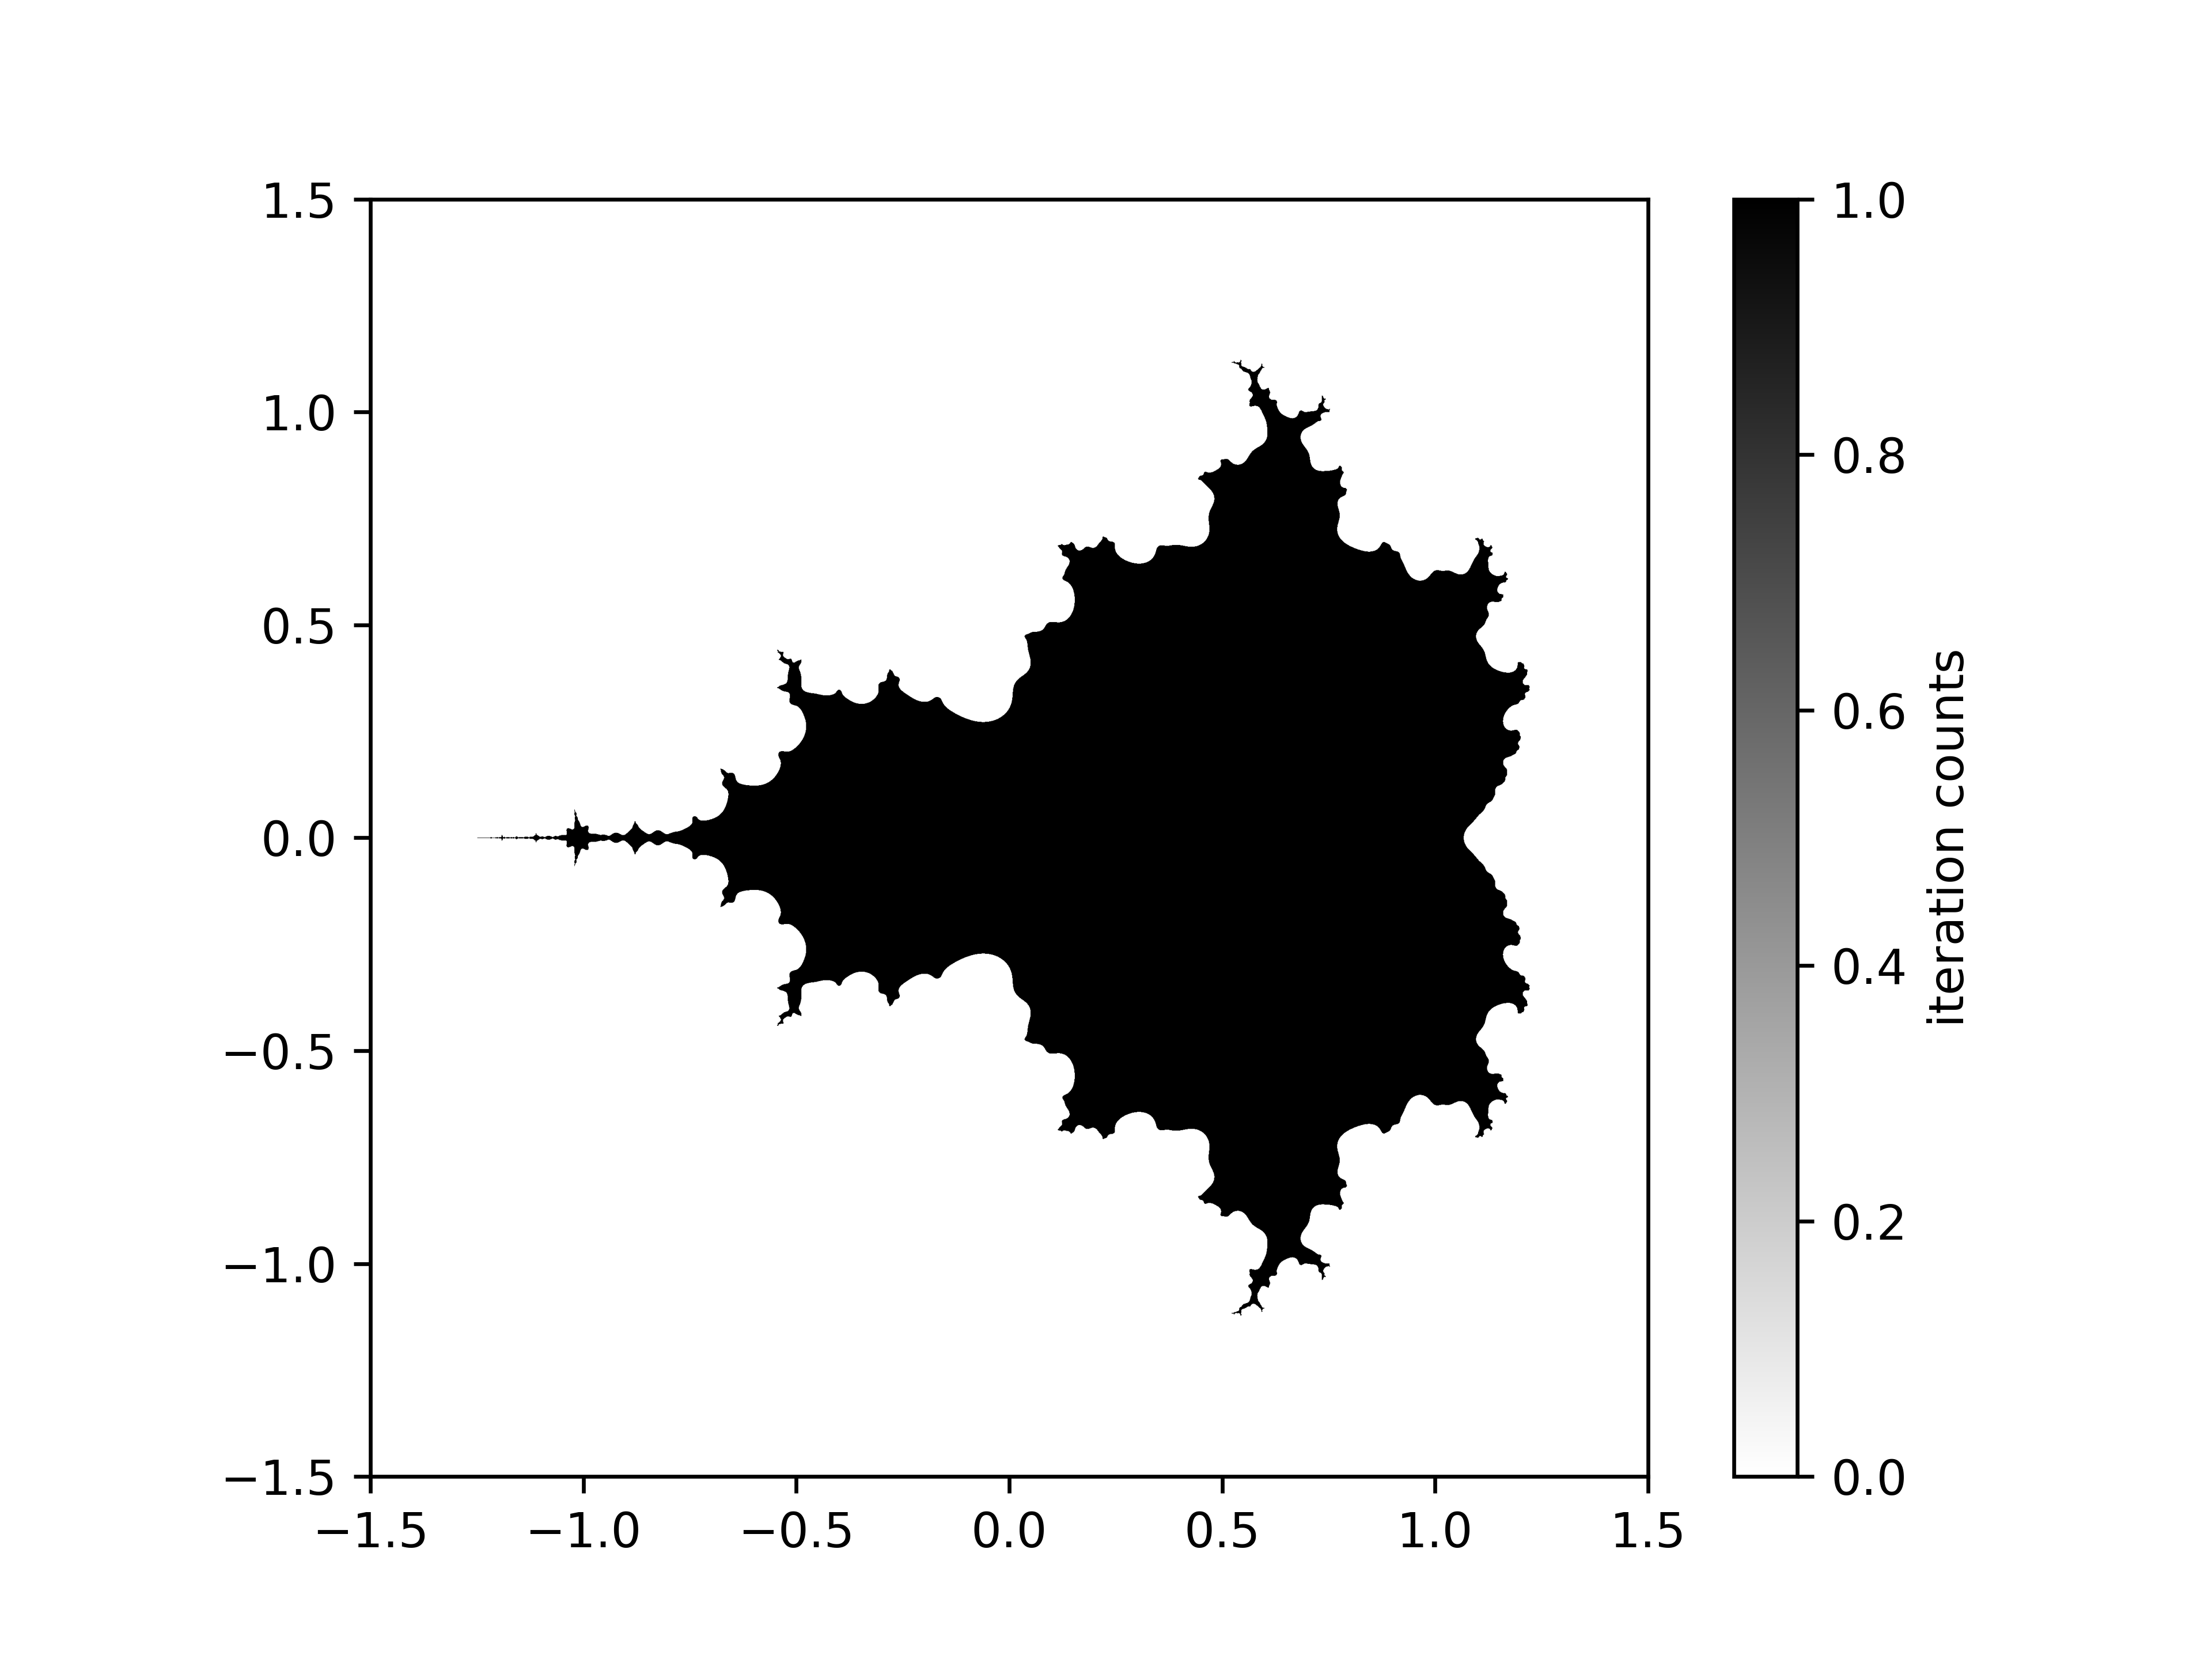
\includegraphics[width=.45\textwidth]{./png/man_normal_n10.png}
		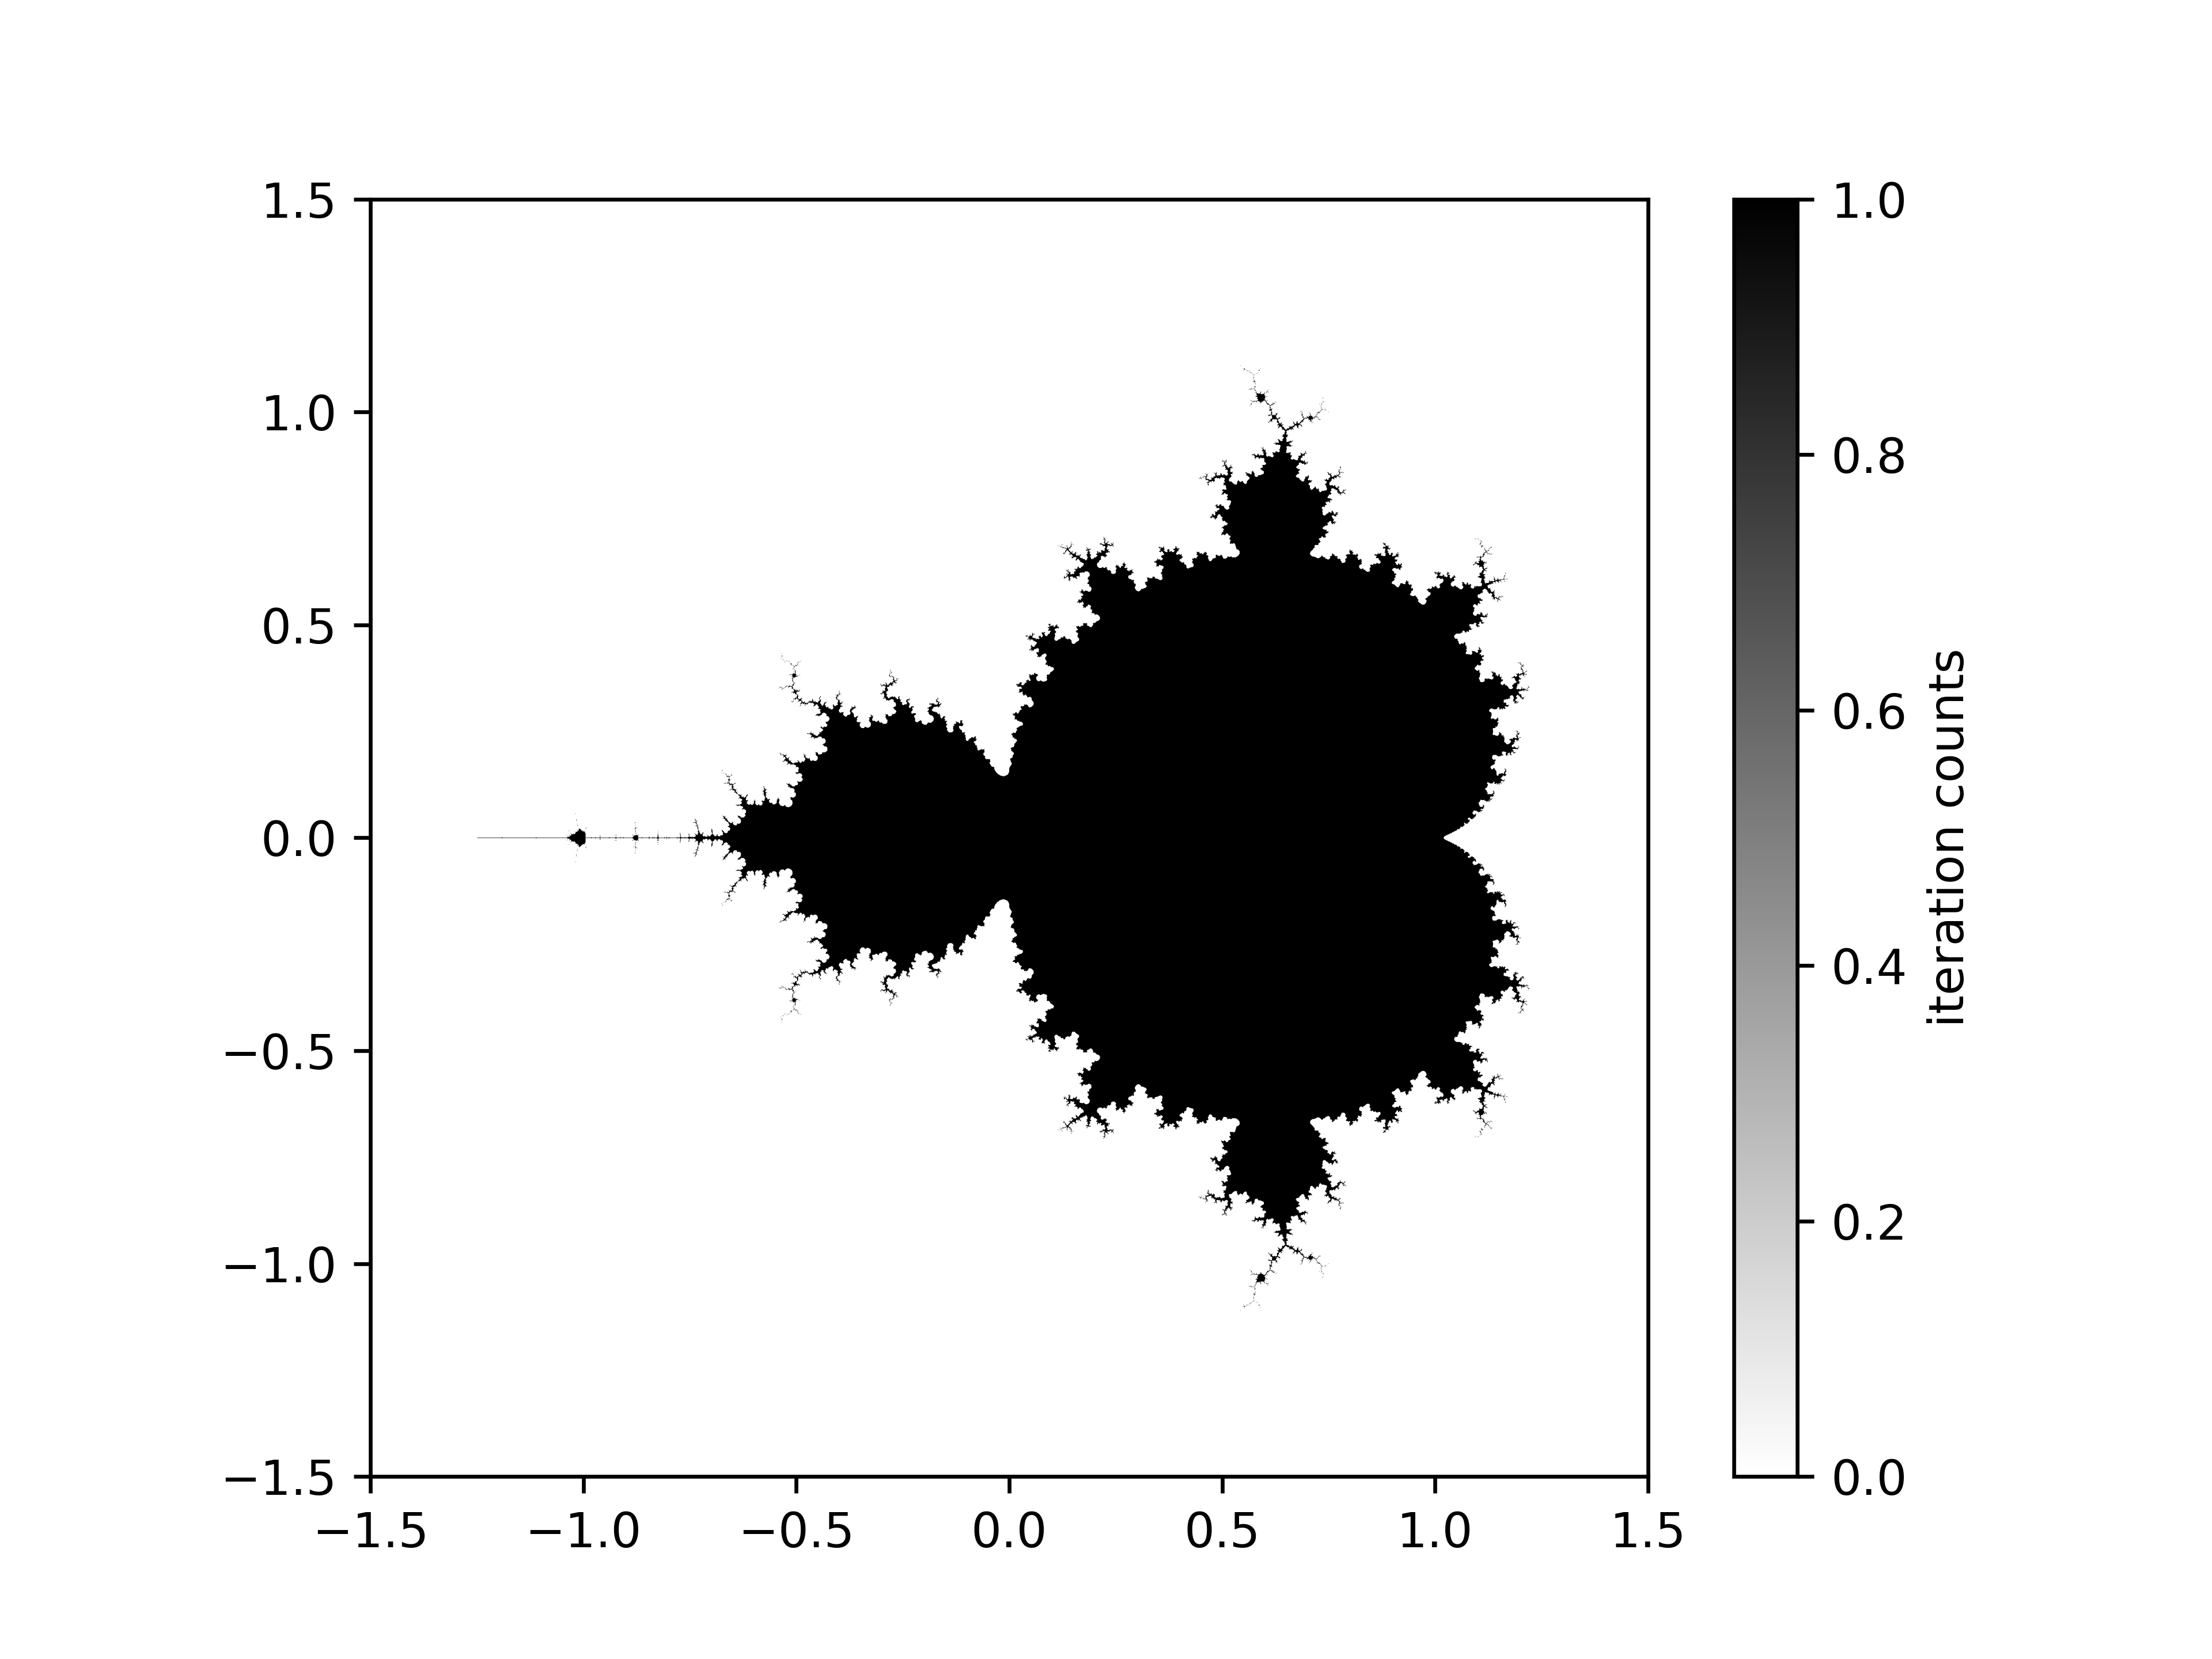
\includegraphics[width=.45\textwidth]{./png/man_normal_n20.png}
		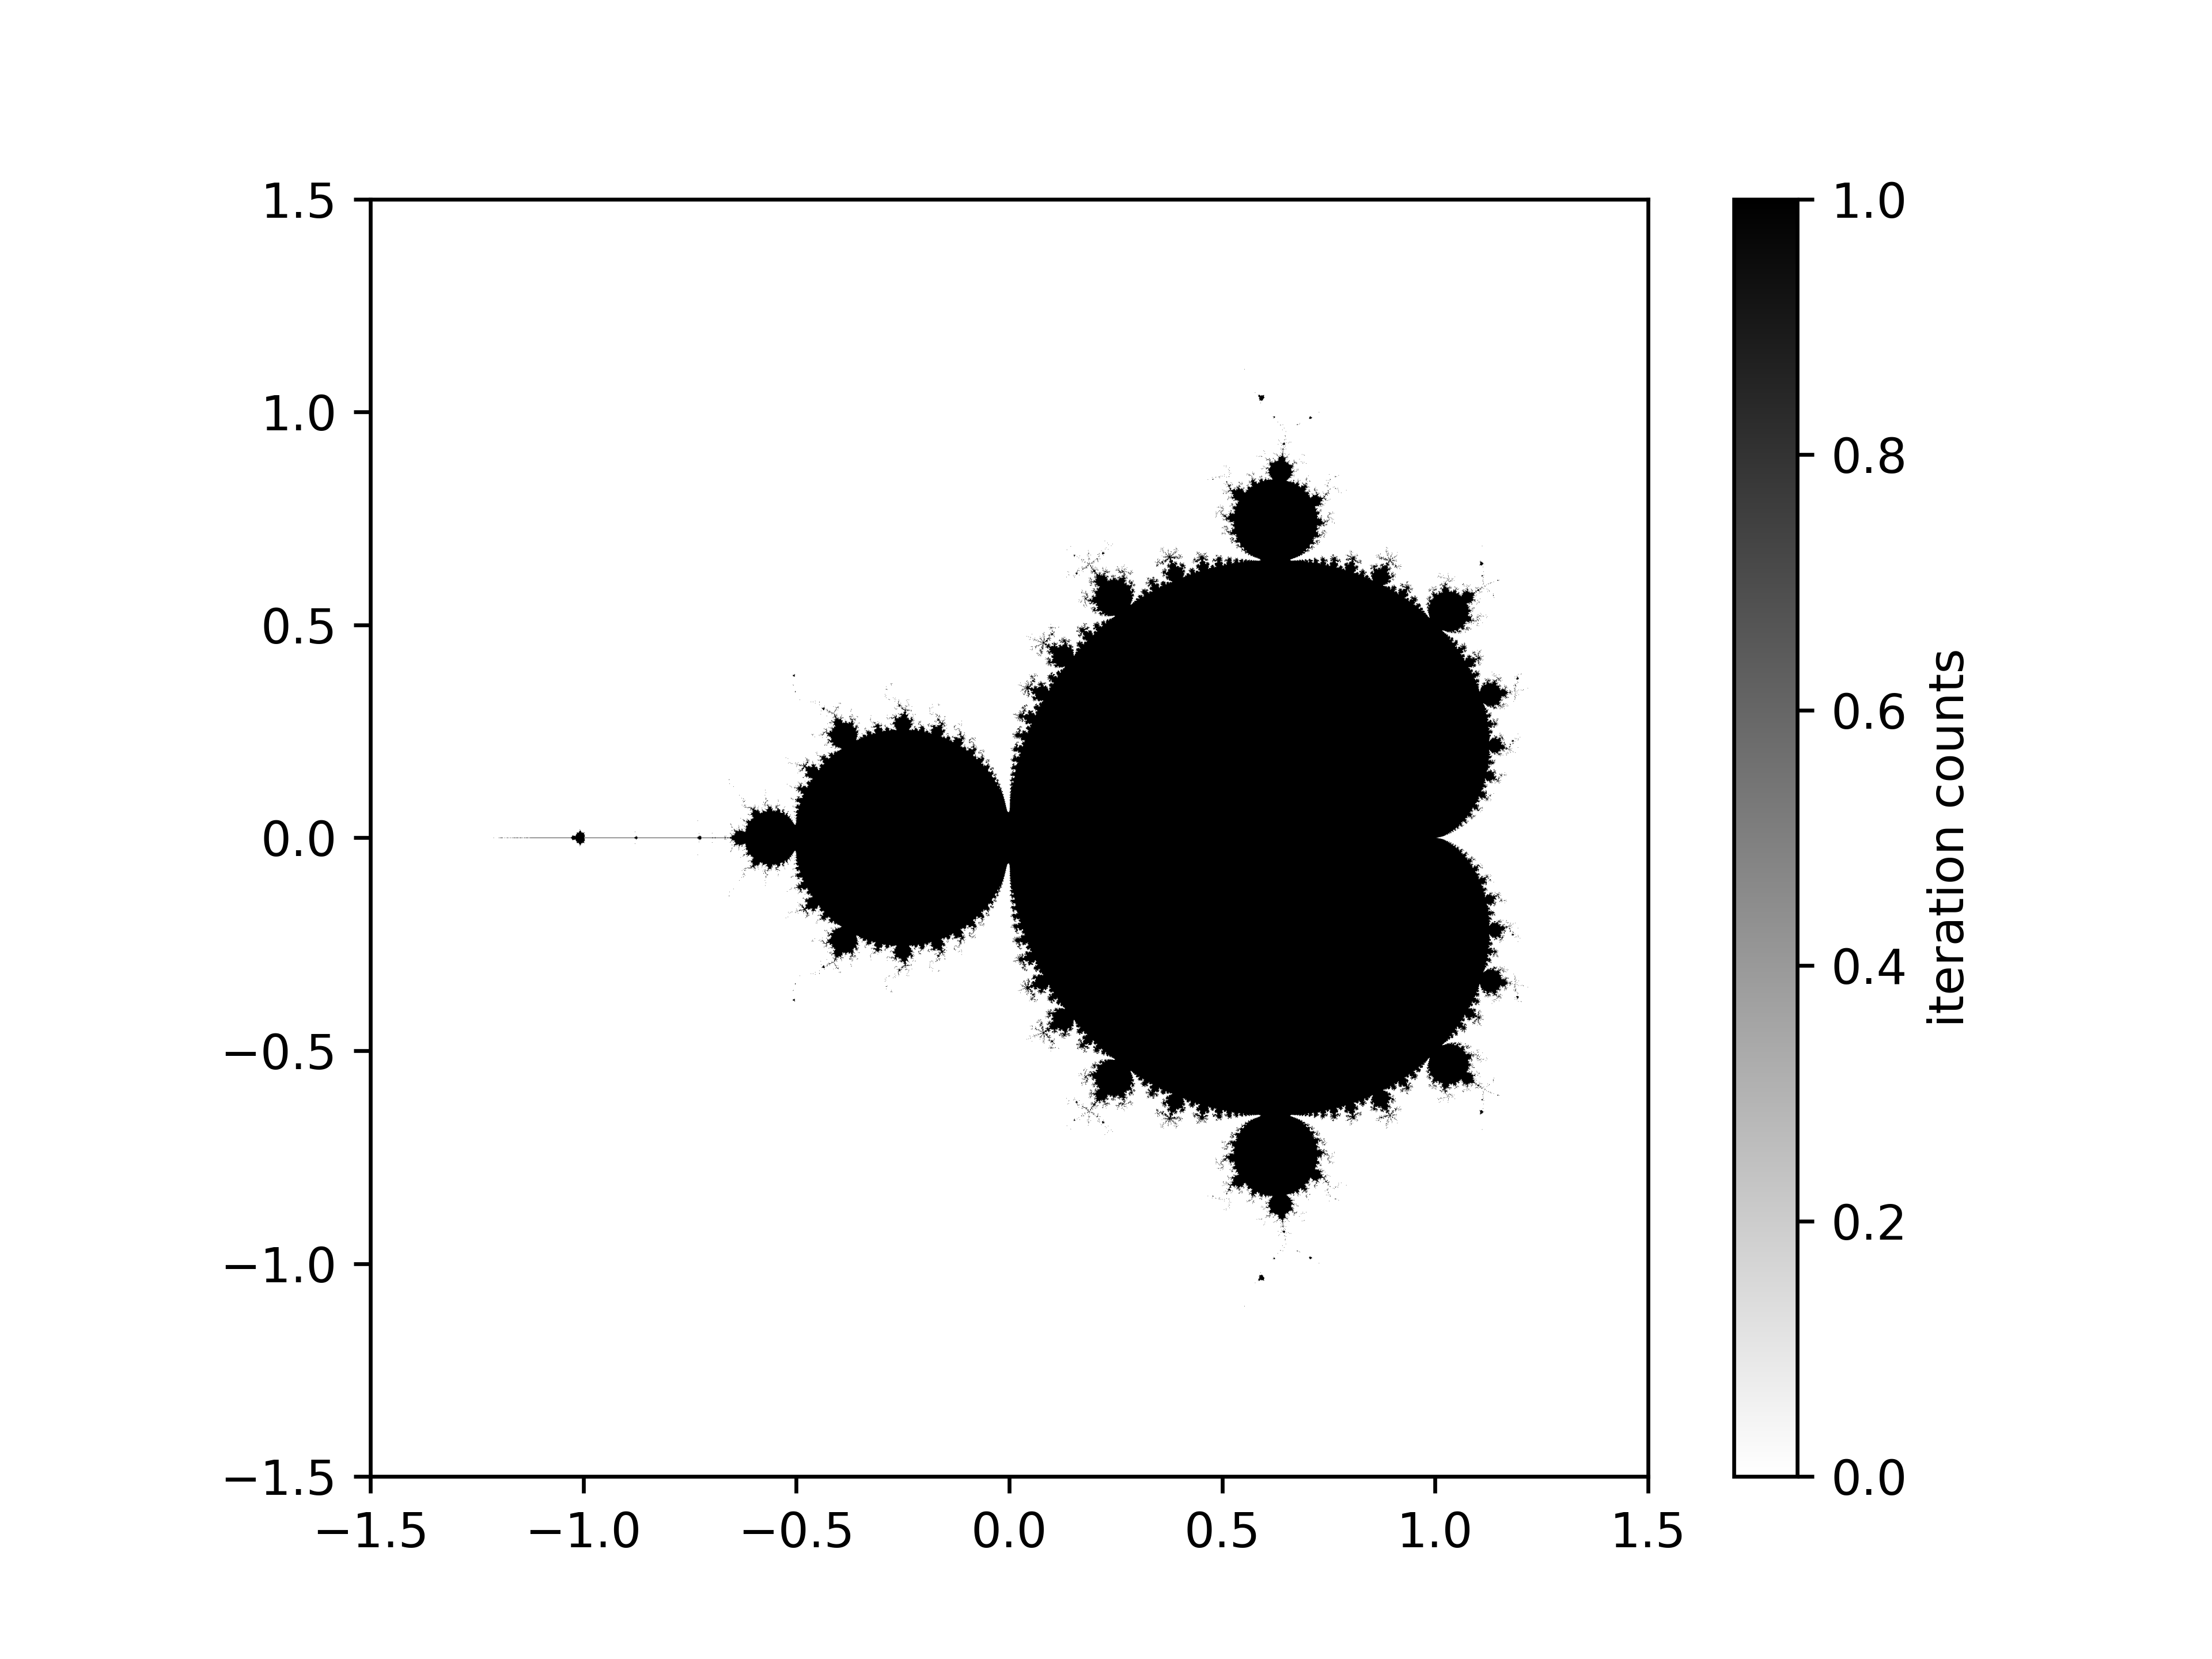
\includegraphics[width=.45\textwidth]{./png/man_normal_n50.png}
		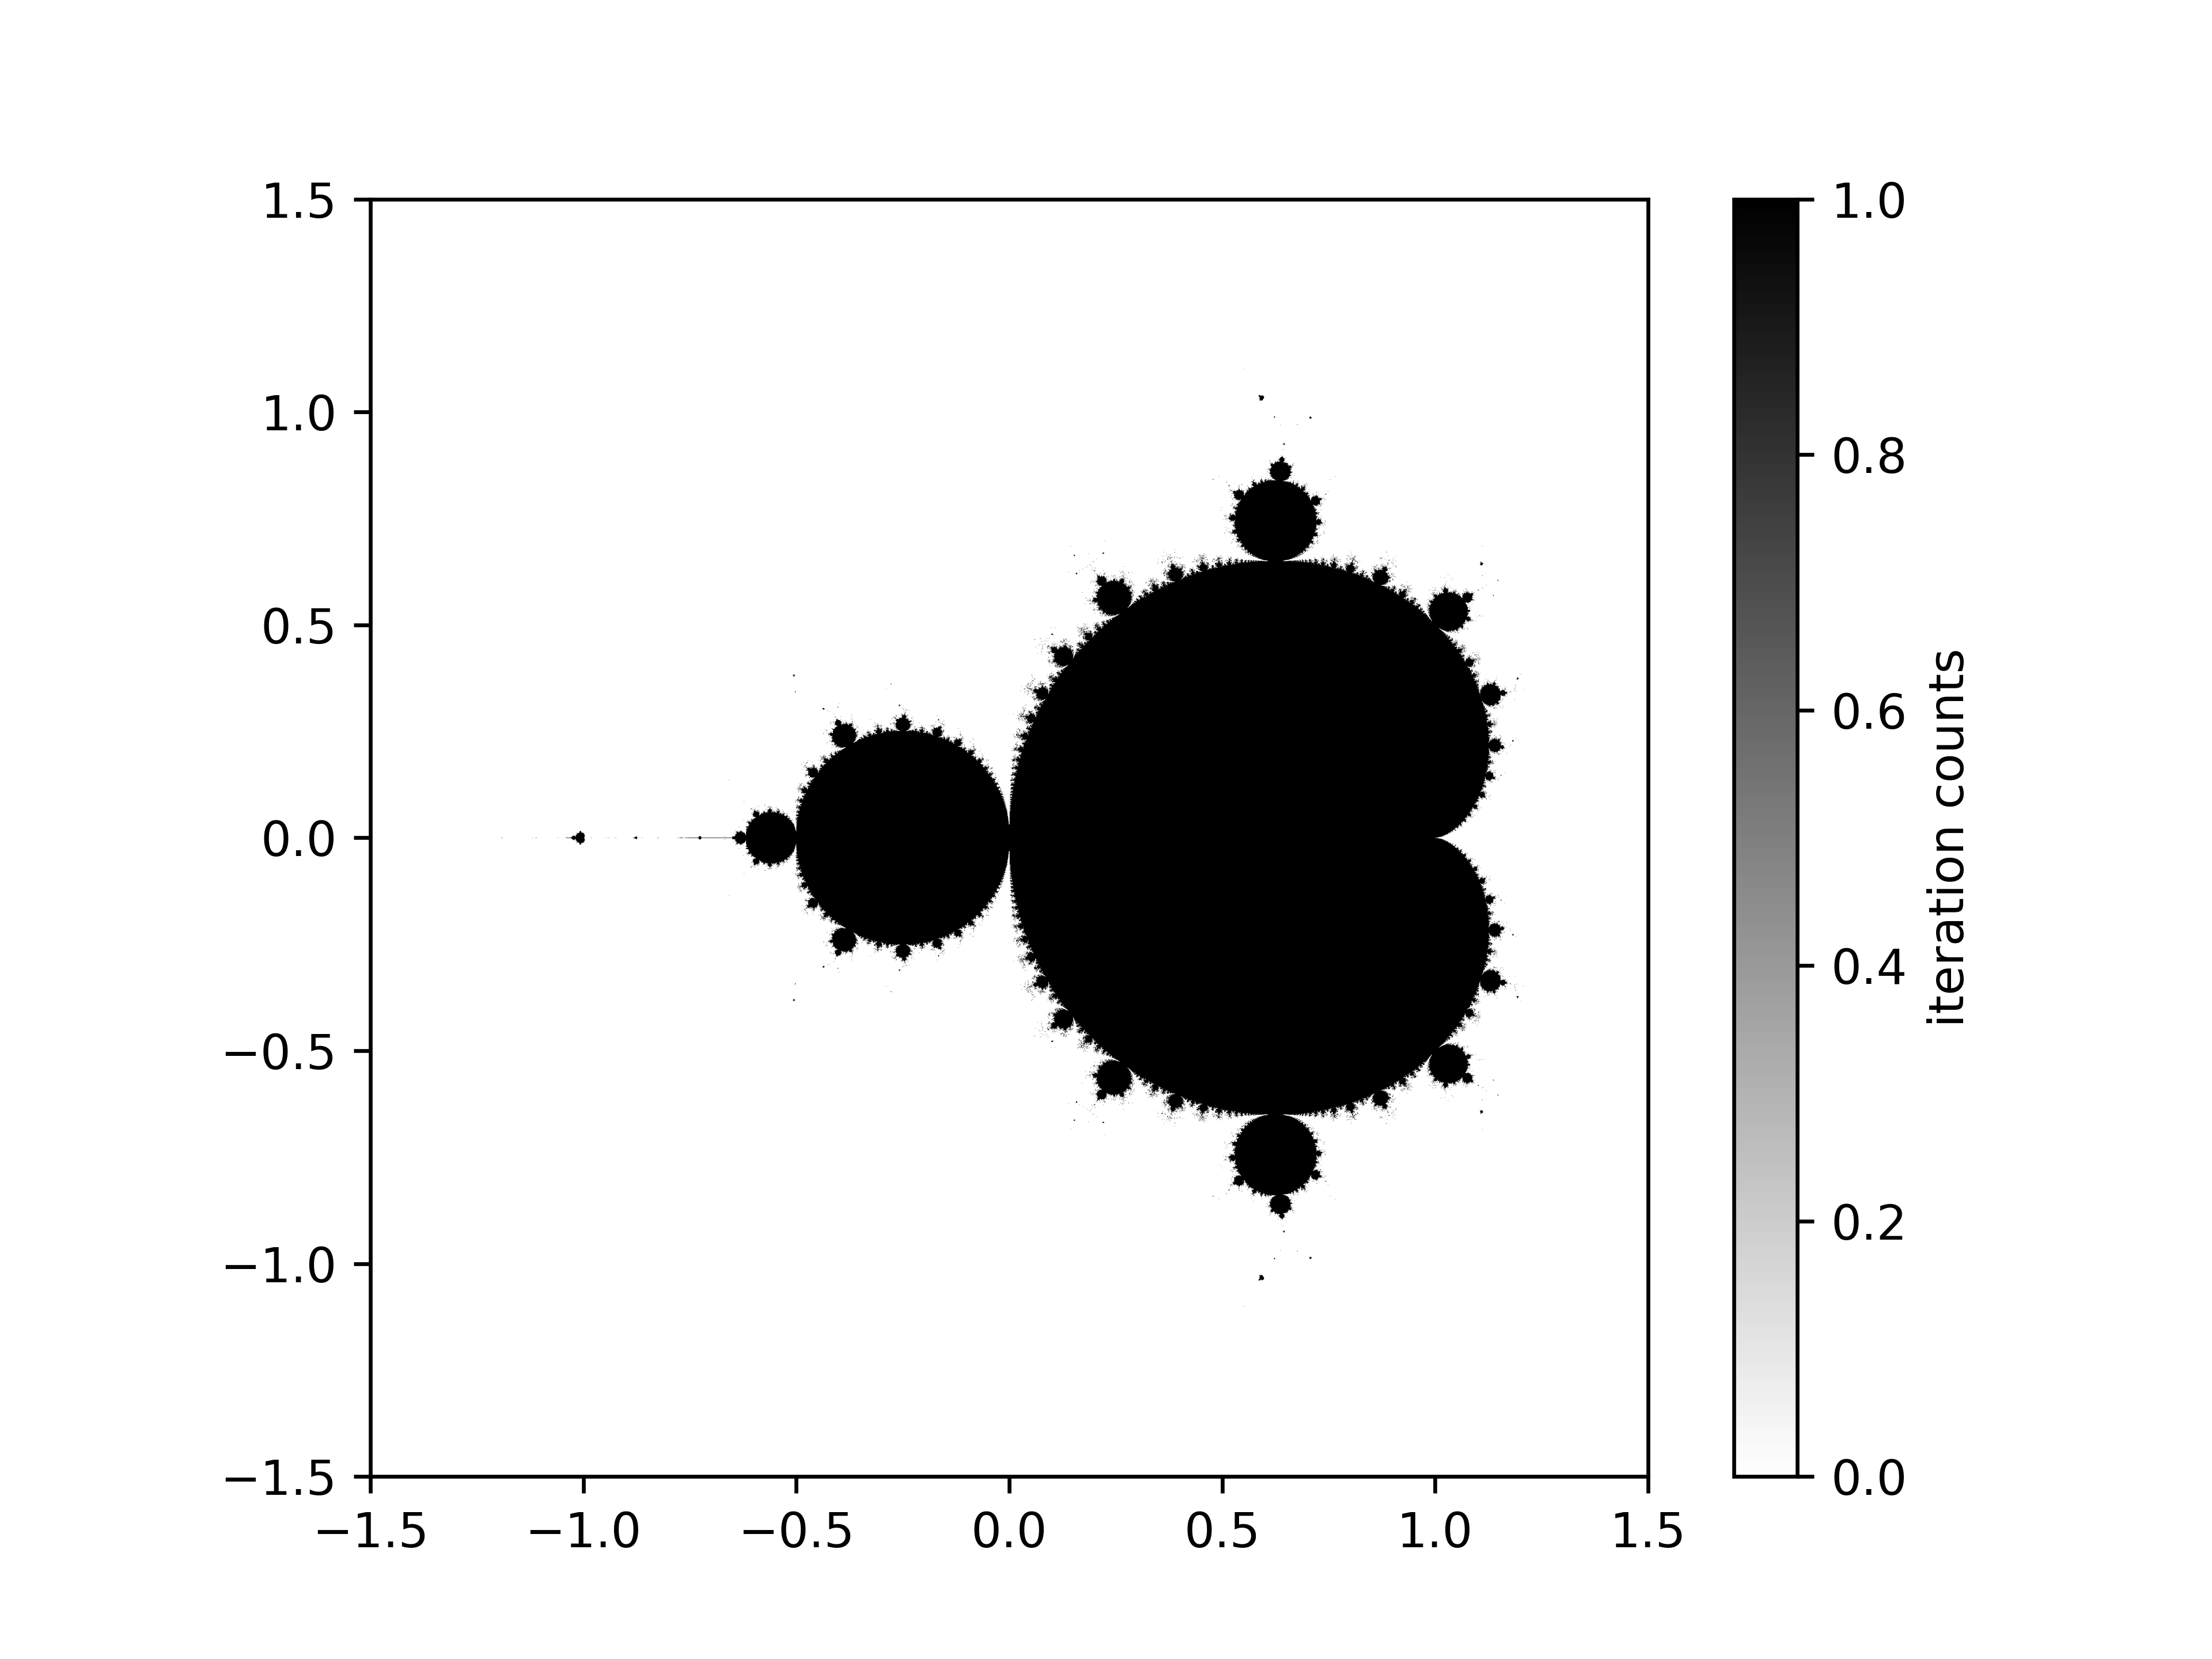
\includegraphics[width=.45\textwidth]{./png/man_normal_n100.png}
		\caption{$N=10,20,50,100$,只对最后一次迭代上色}
		\label{normal}
	\end{figure}

开始使$f$的值与$n$产生联系。
\item 令$f(n,z)=n$,再分别取$N=10,20,50,100$:
\begin{figure}[H]
	\centering
	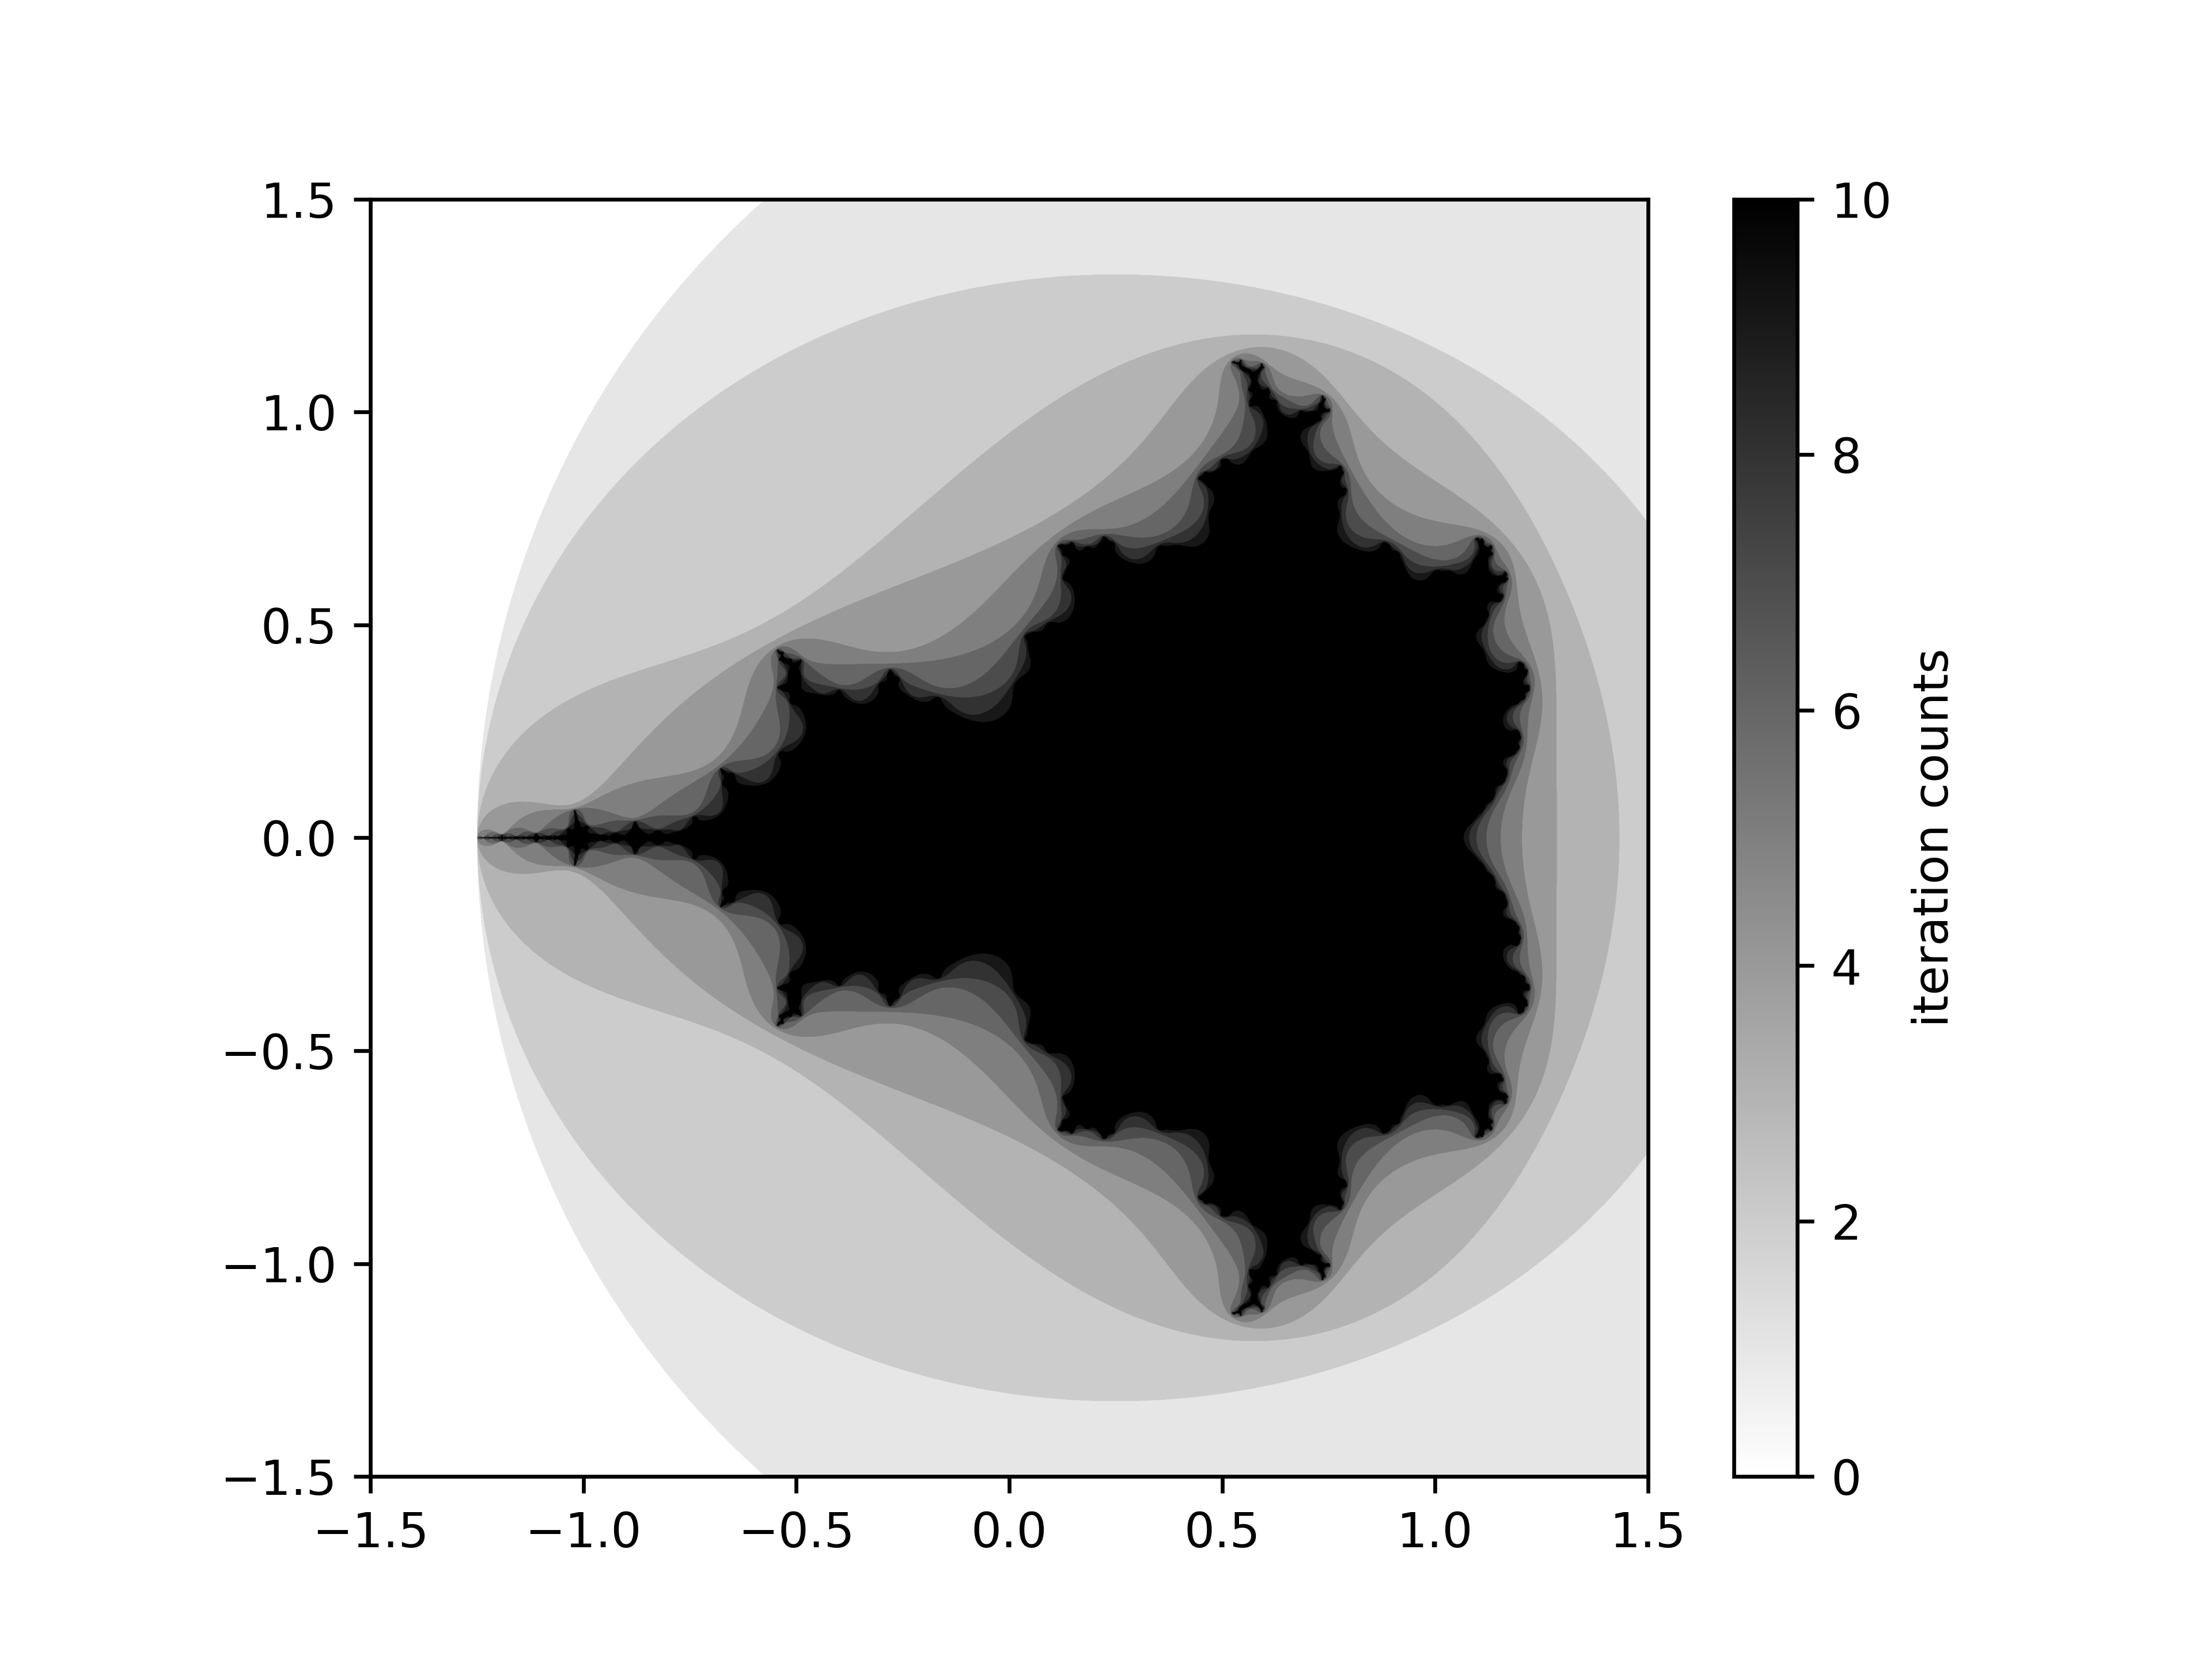
\includegraphics[width=.45\textwidth]{./png/man_complex_n10.png}
	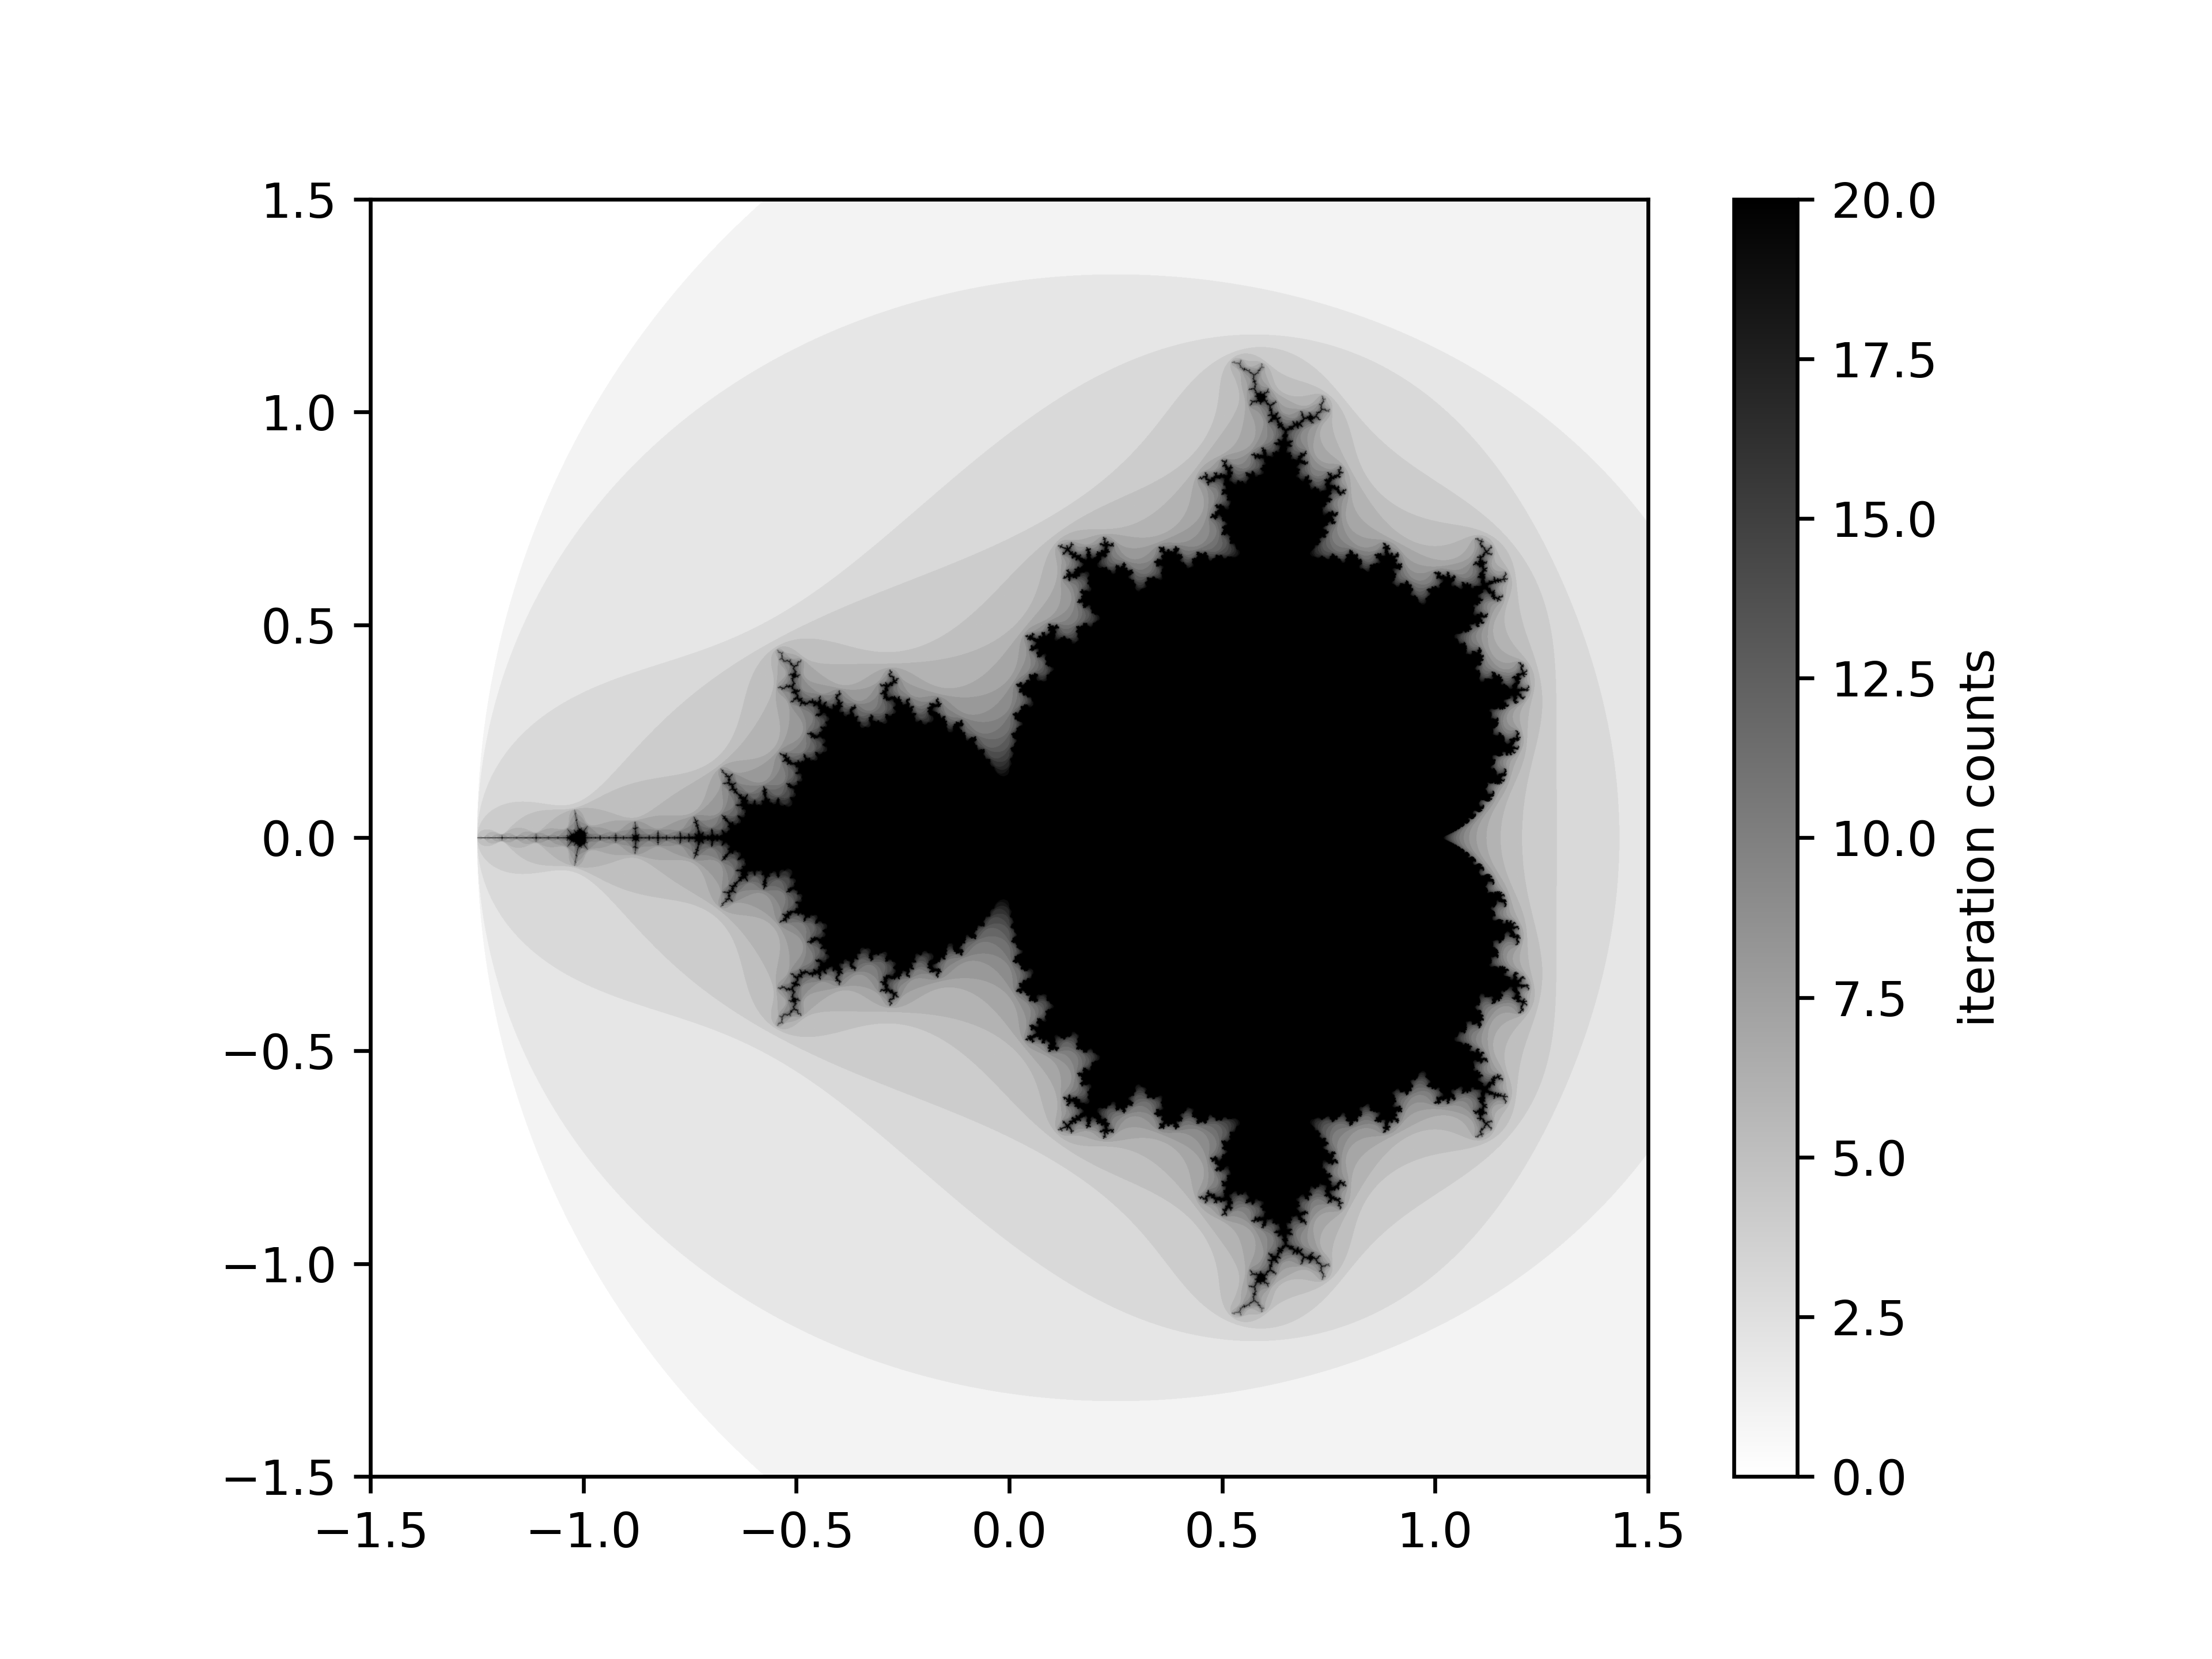
\includegraphics[width=.45\textwidth]{./png/man_complex_n20.png}
	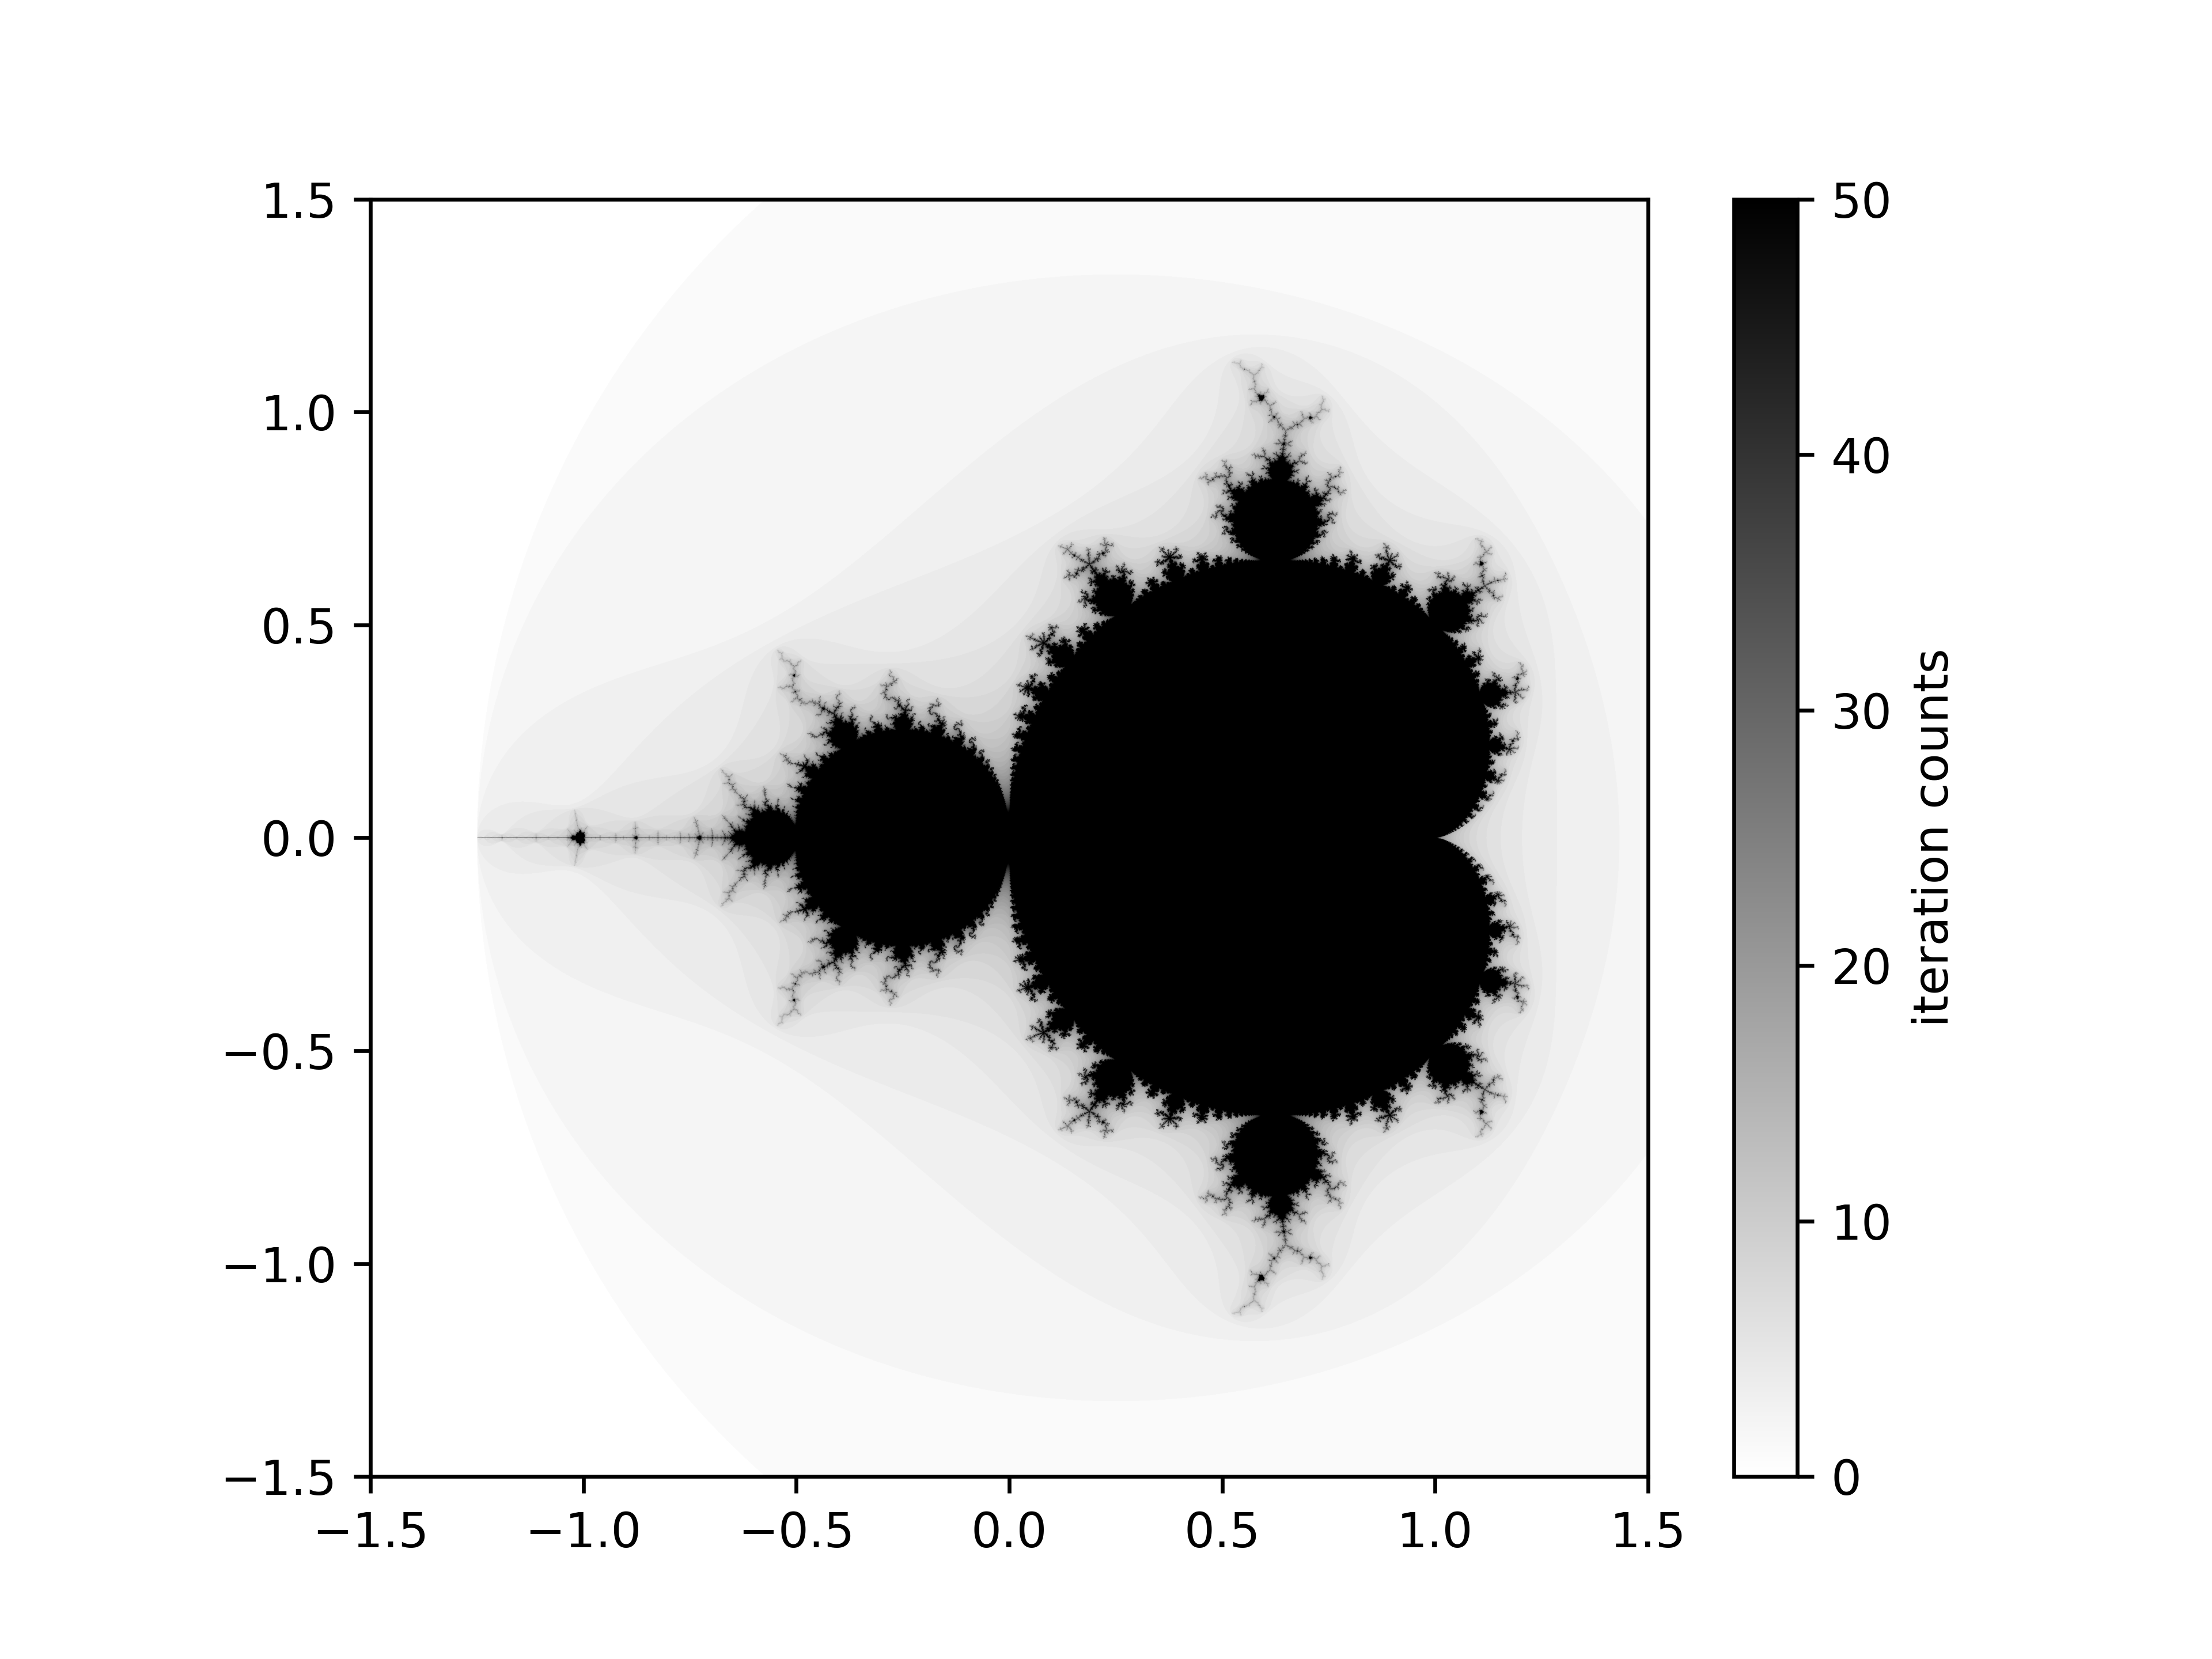
\includegraphics[width=.45\textwidth]{./png/man_complex_n50.png}
	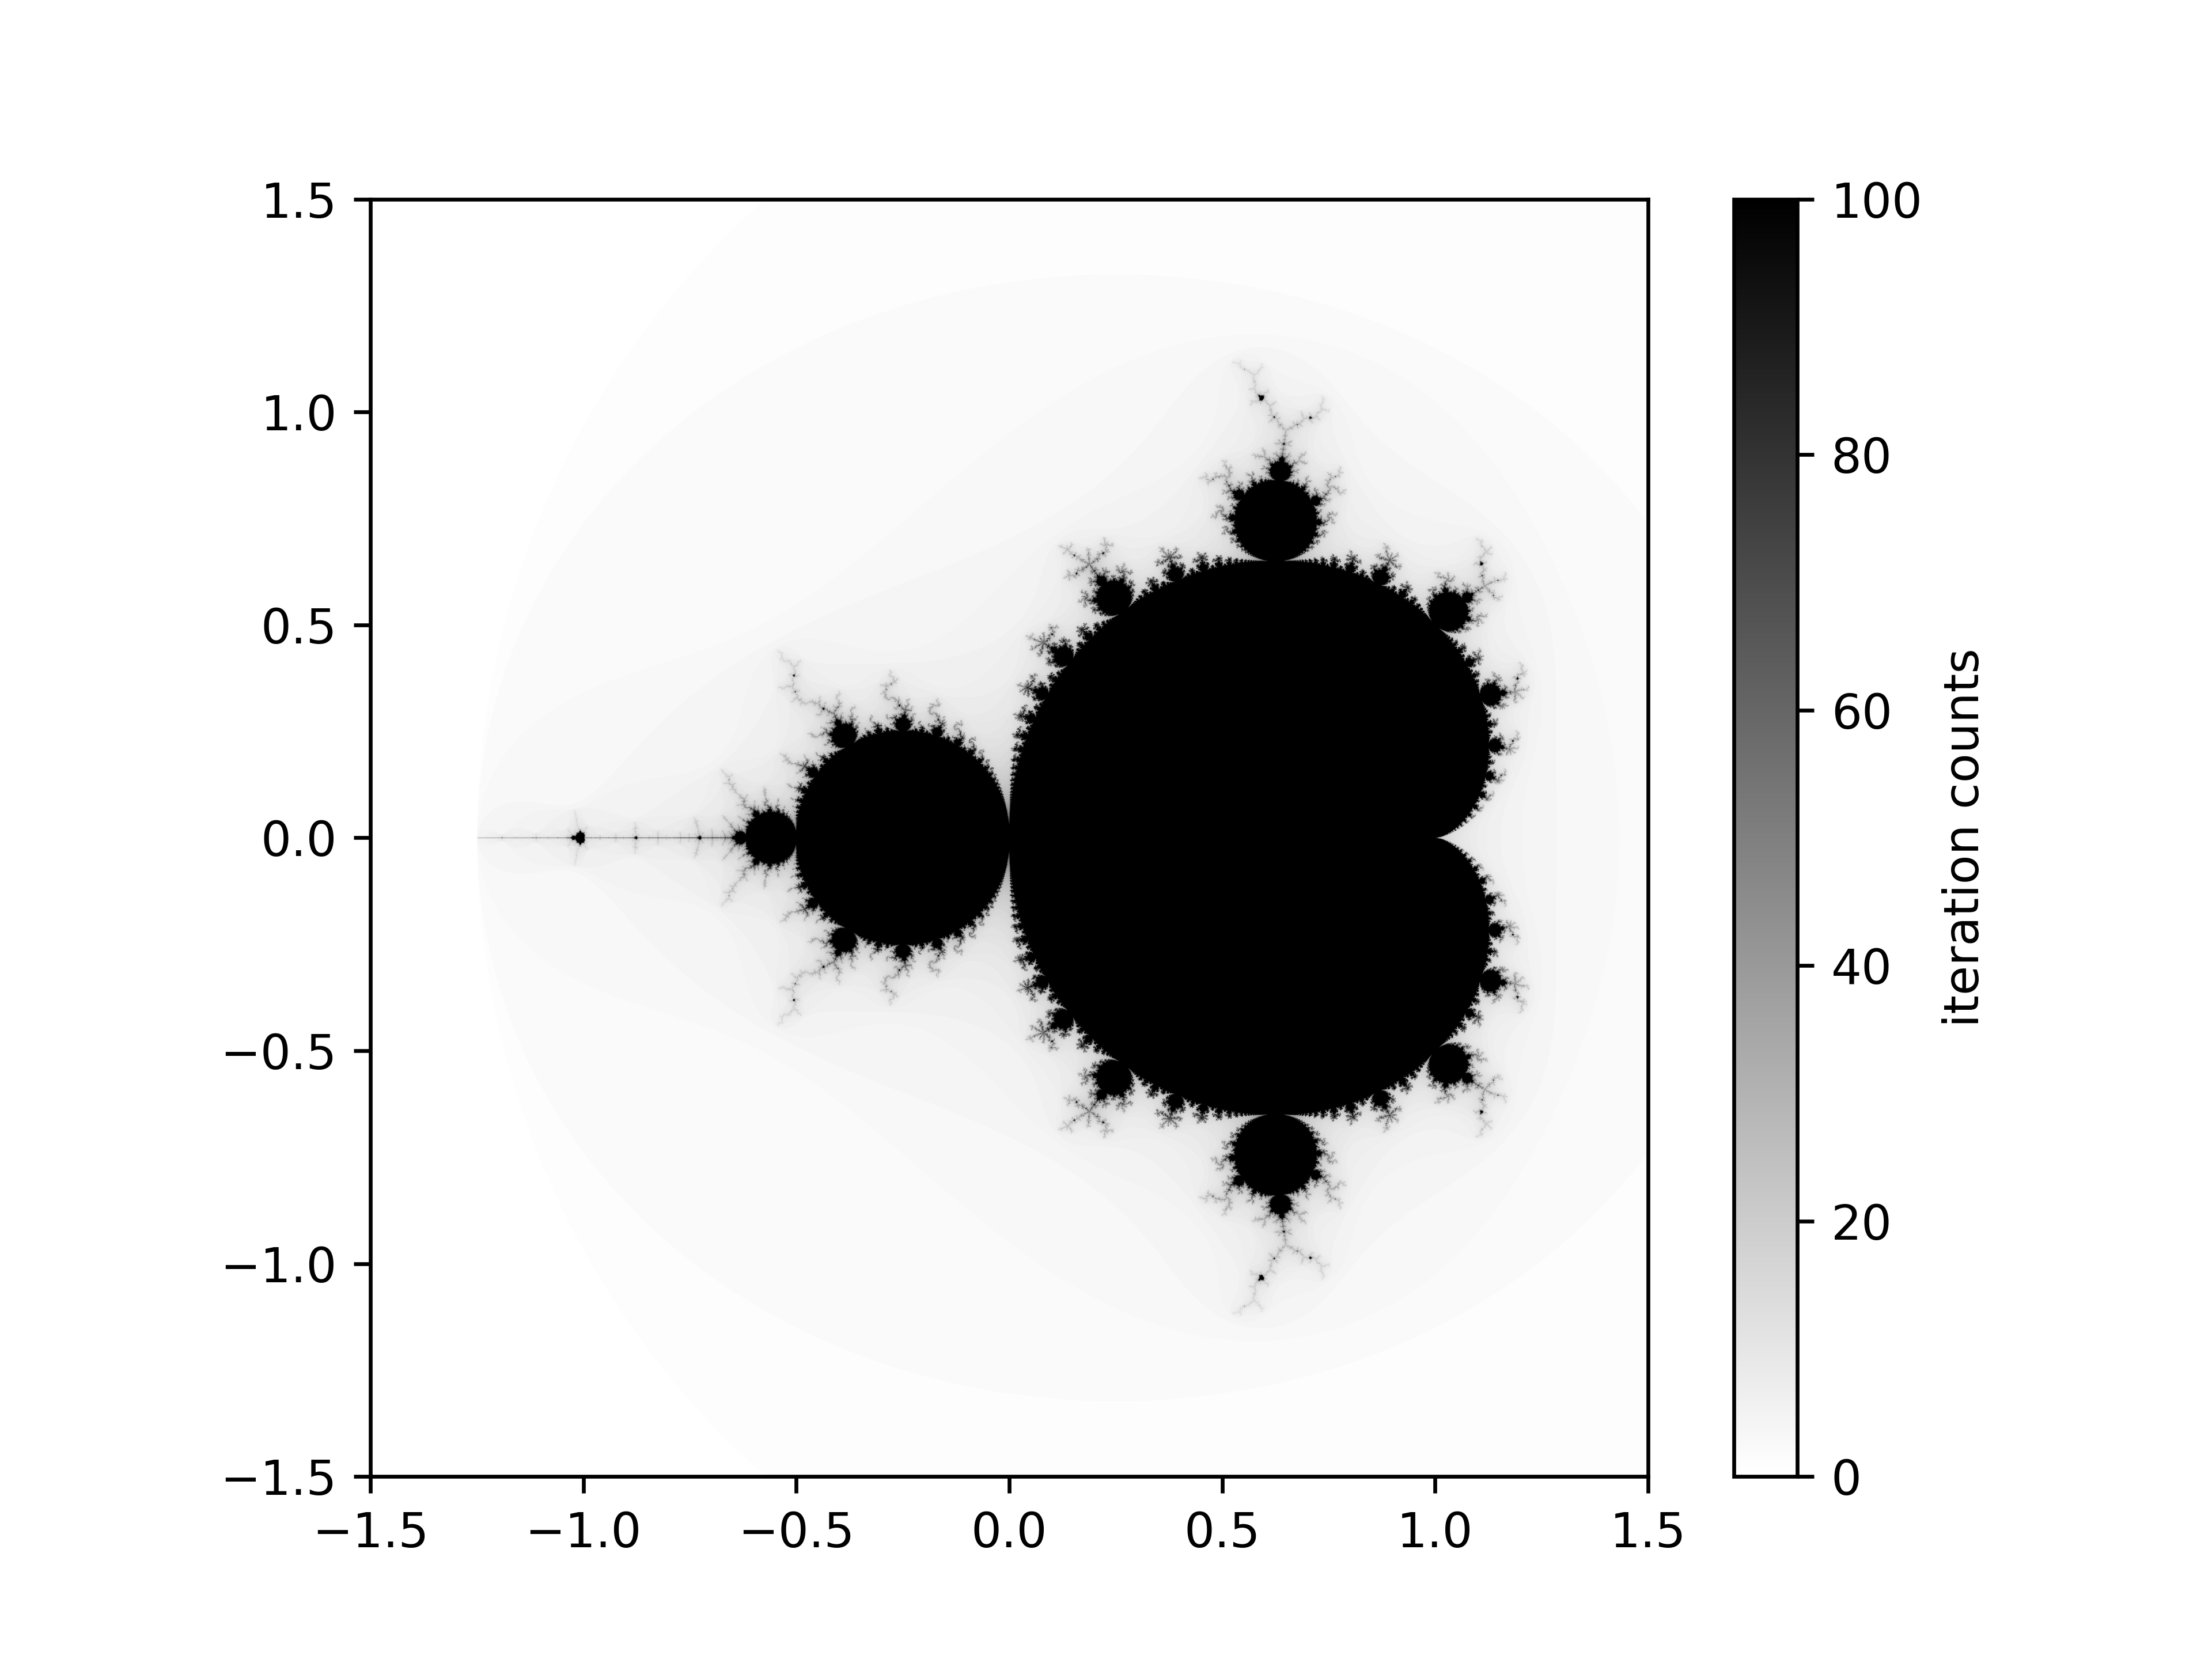
\includegraphics[width=.45\textwidth]{./png/man_complex_n100.png}
	\caption{$N=10,20,50,100$,每迭代一次颜色加深一点}
	\label{complex}
\end{figure}
\item 在类似\ref{complex}的情形下把灰度图改为黑白相间图($f(n,z)=(-1)^i$)和彩图:
\begin{figure}[H]
	\centering
	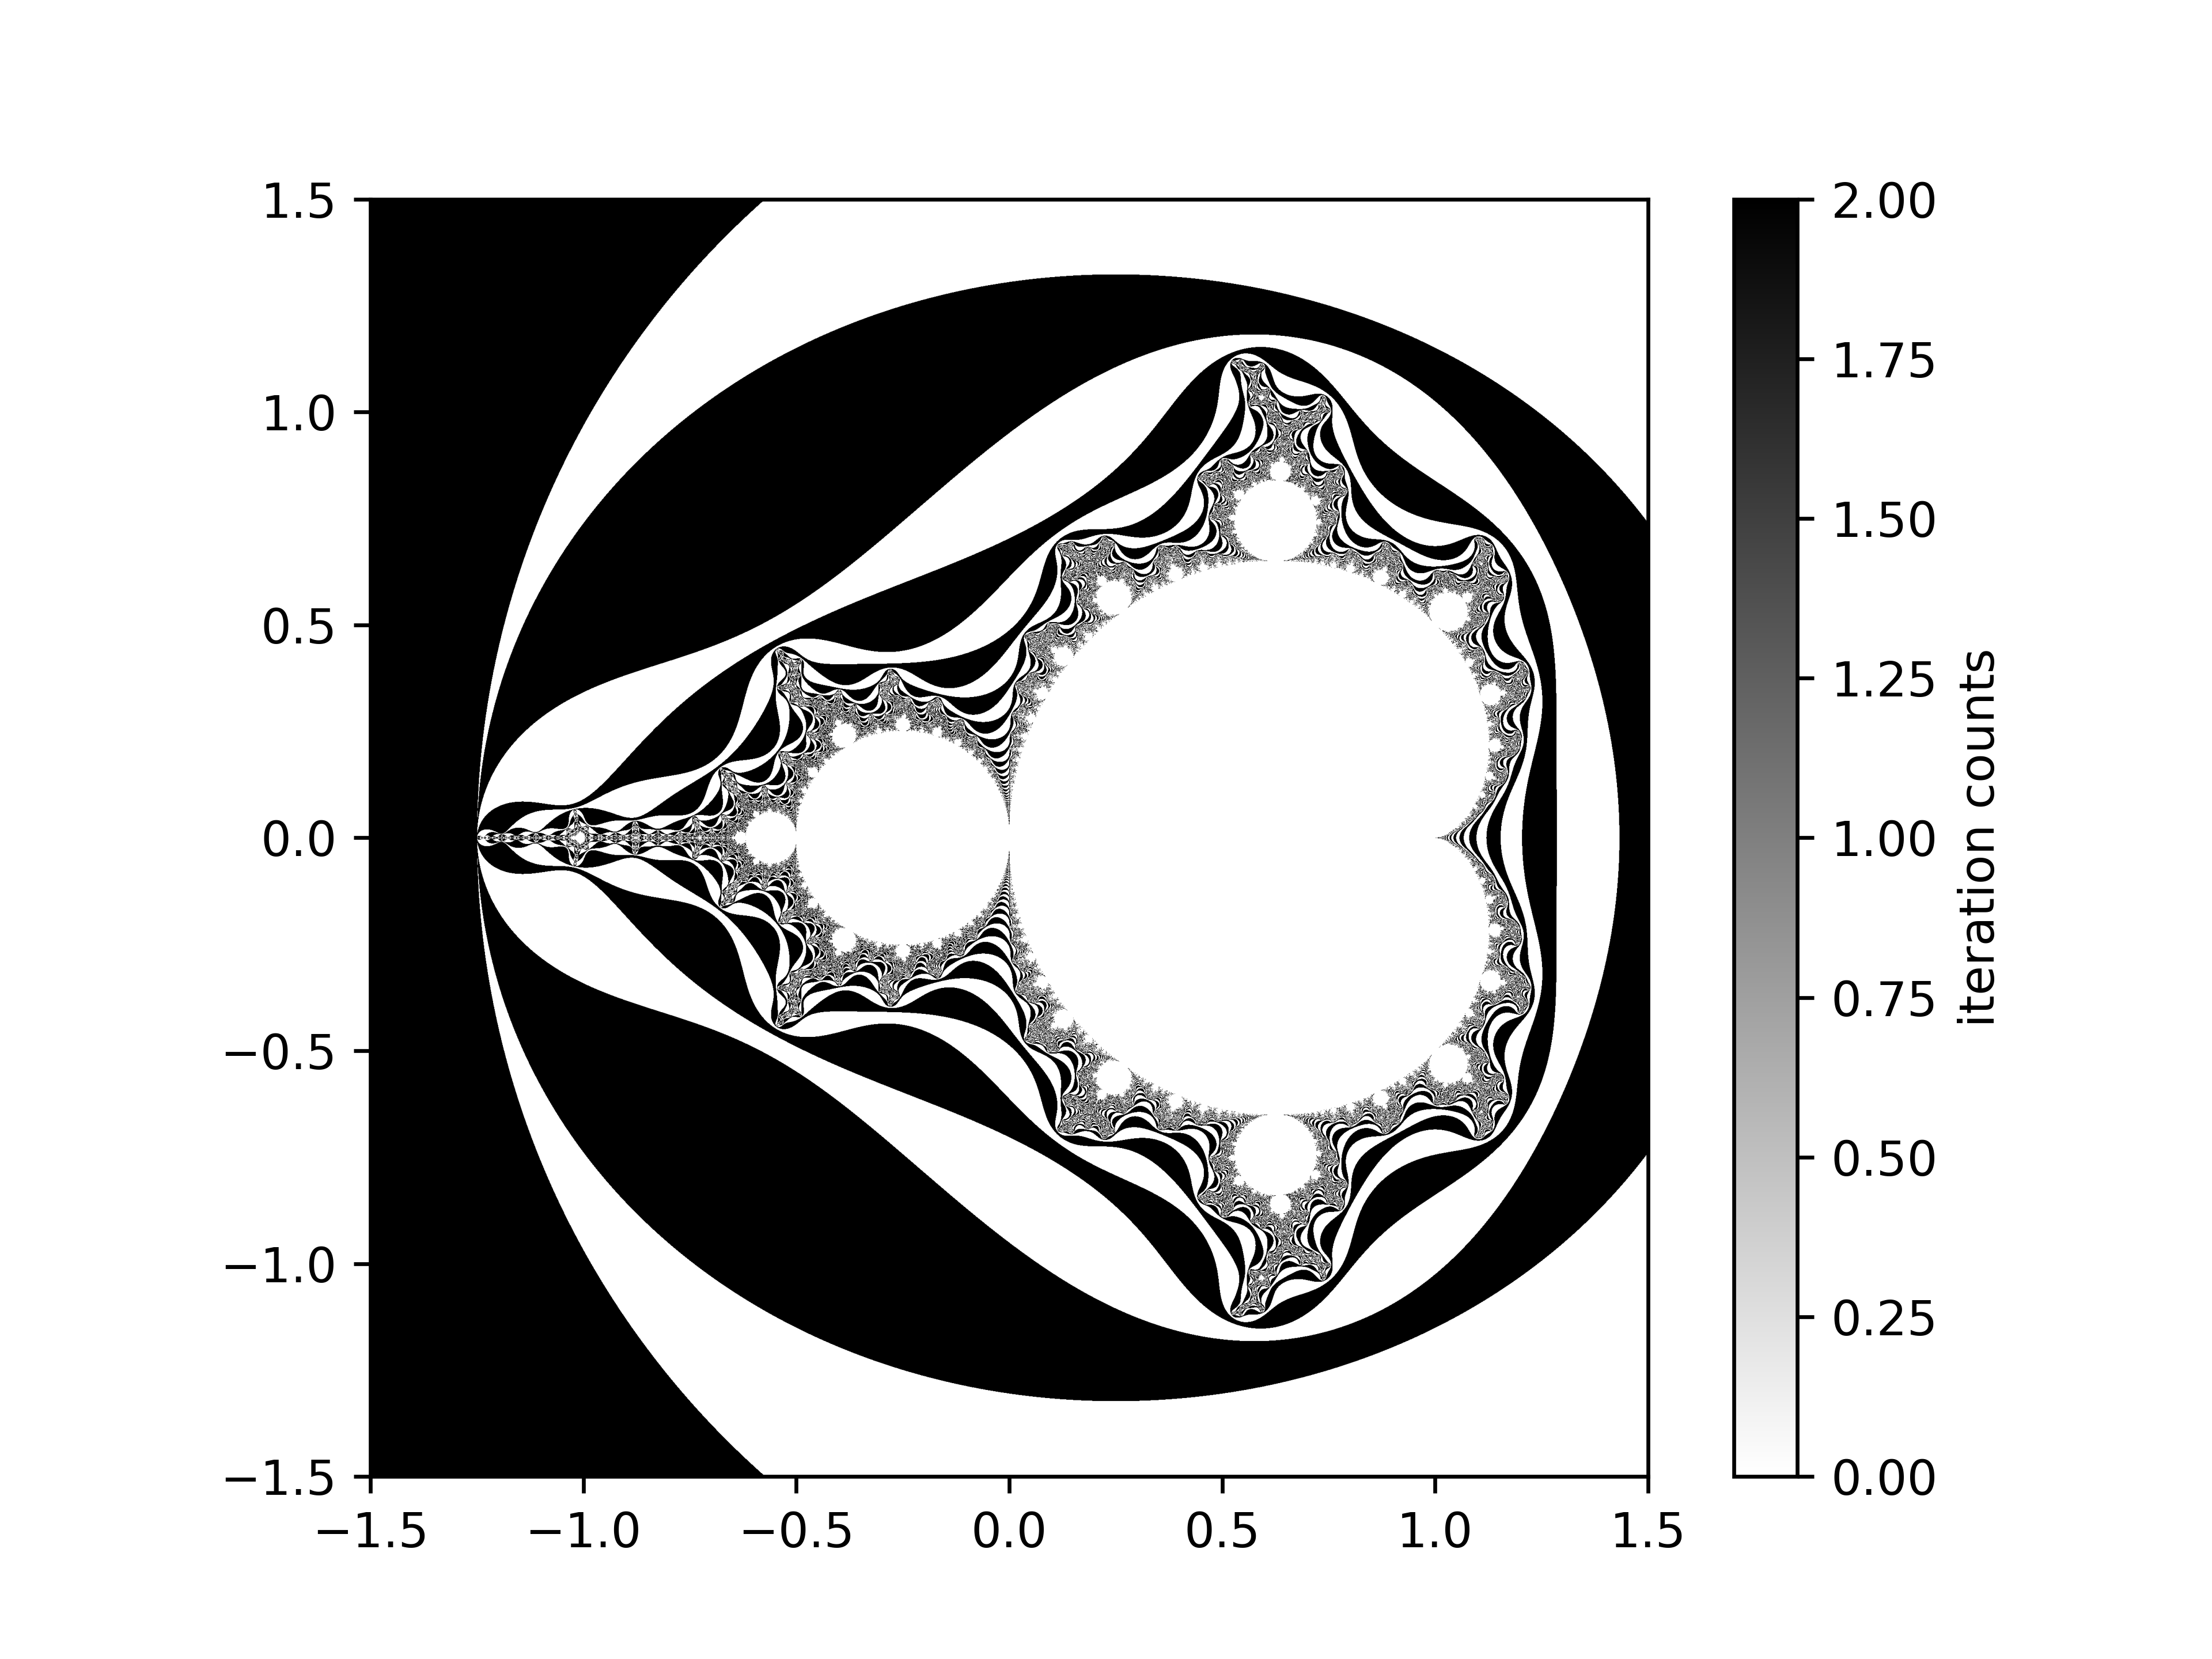
\includegraphics[width=.45\textwidth]{./png/man_amazing_n100.png}
	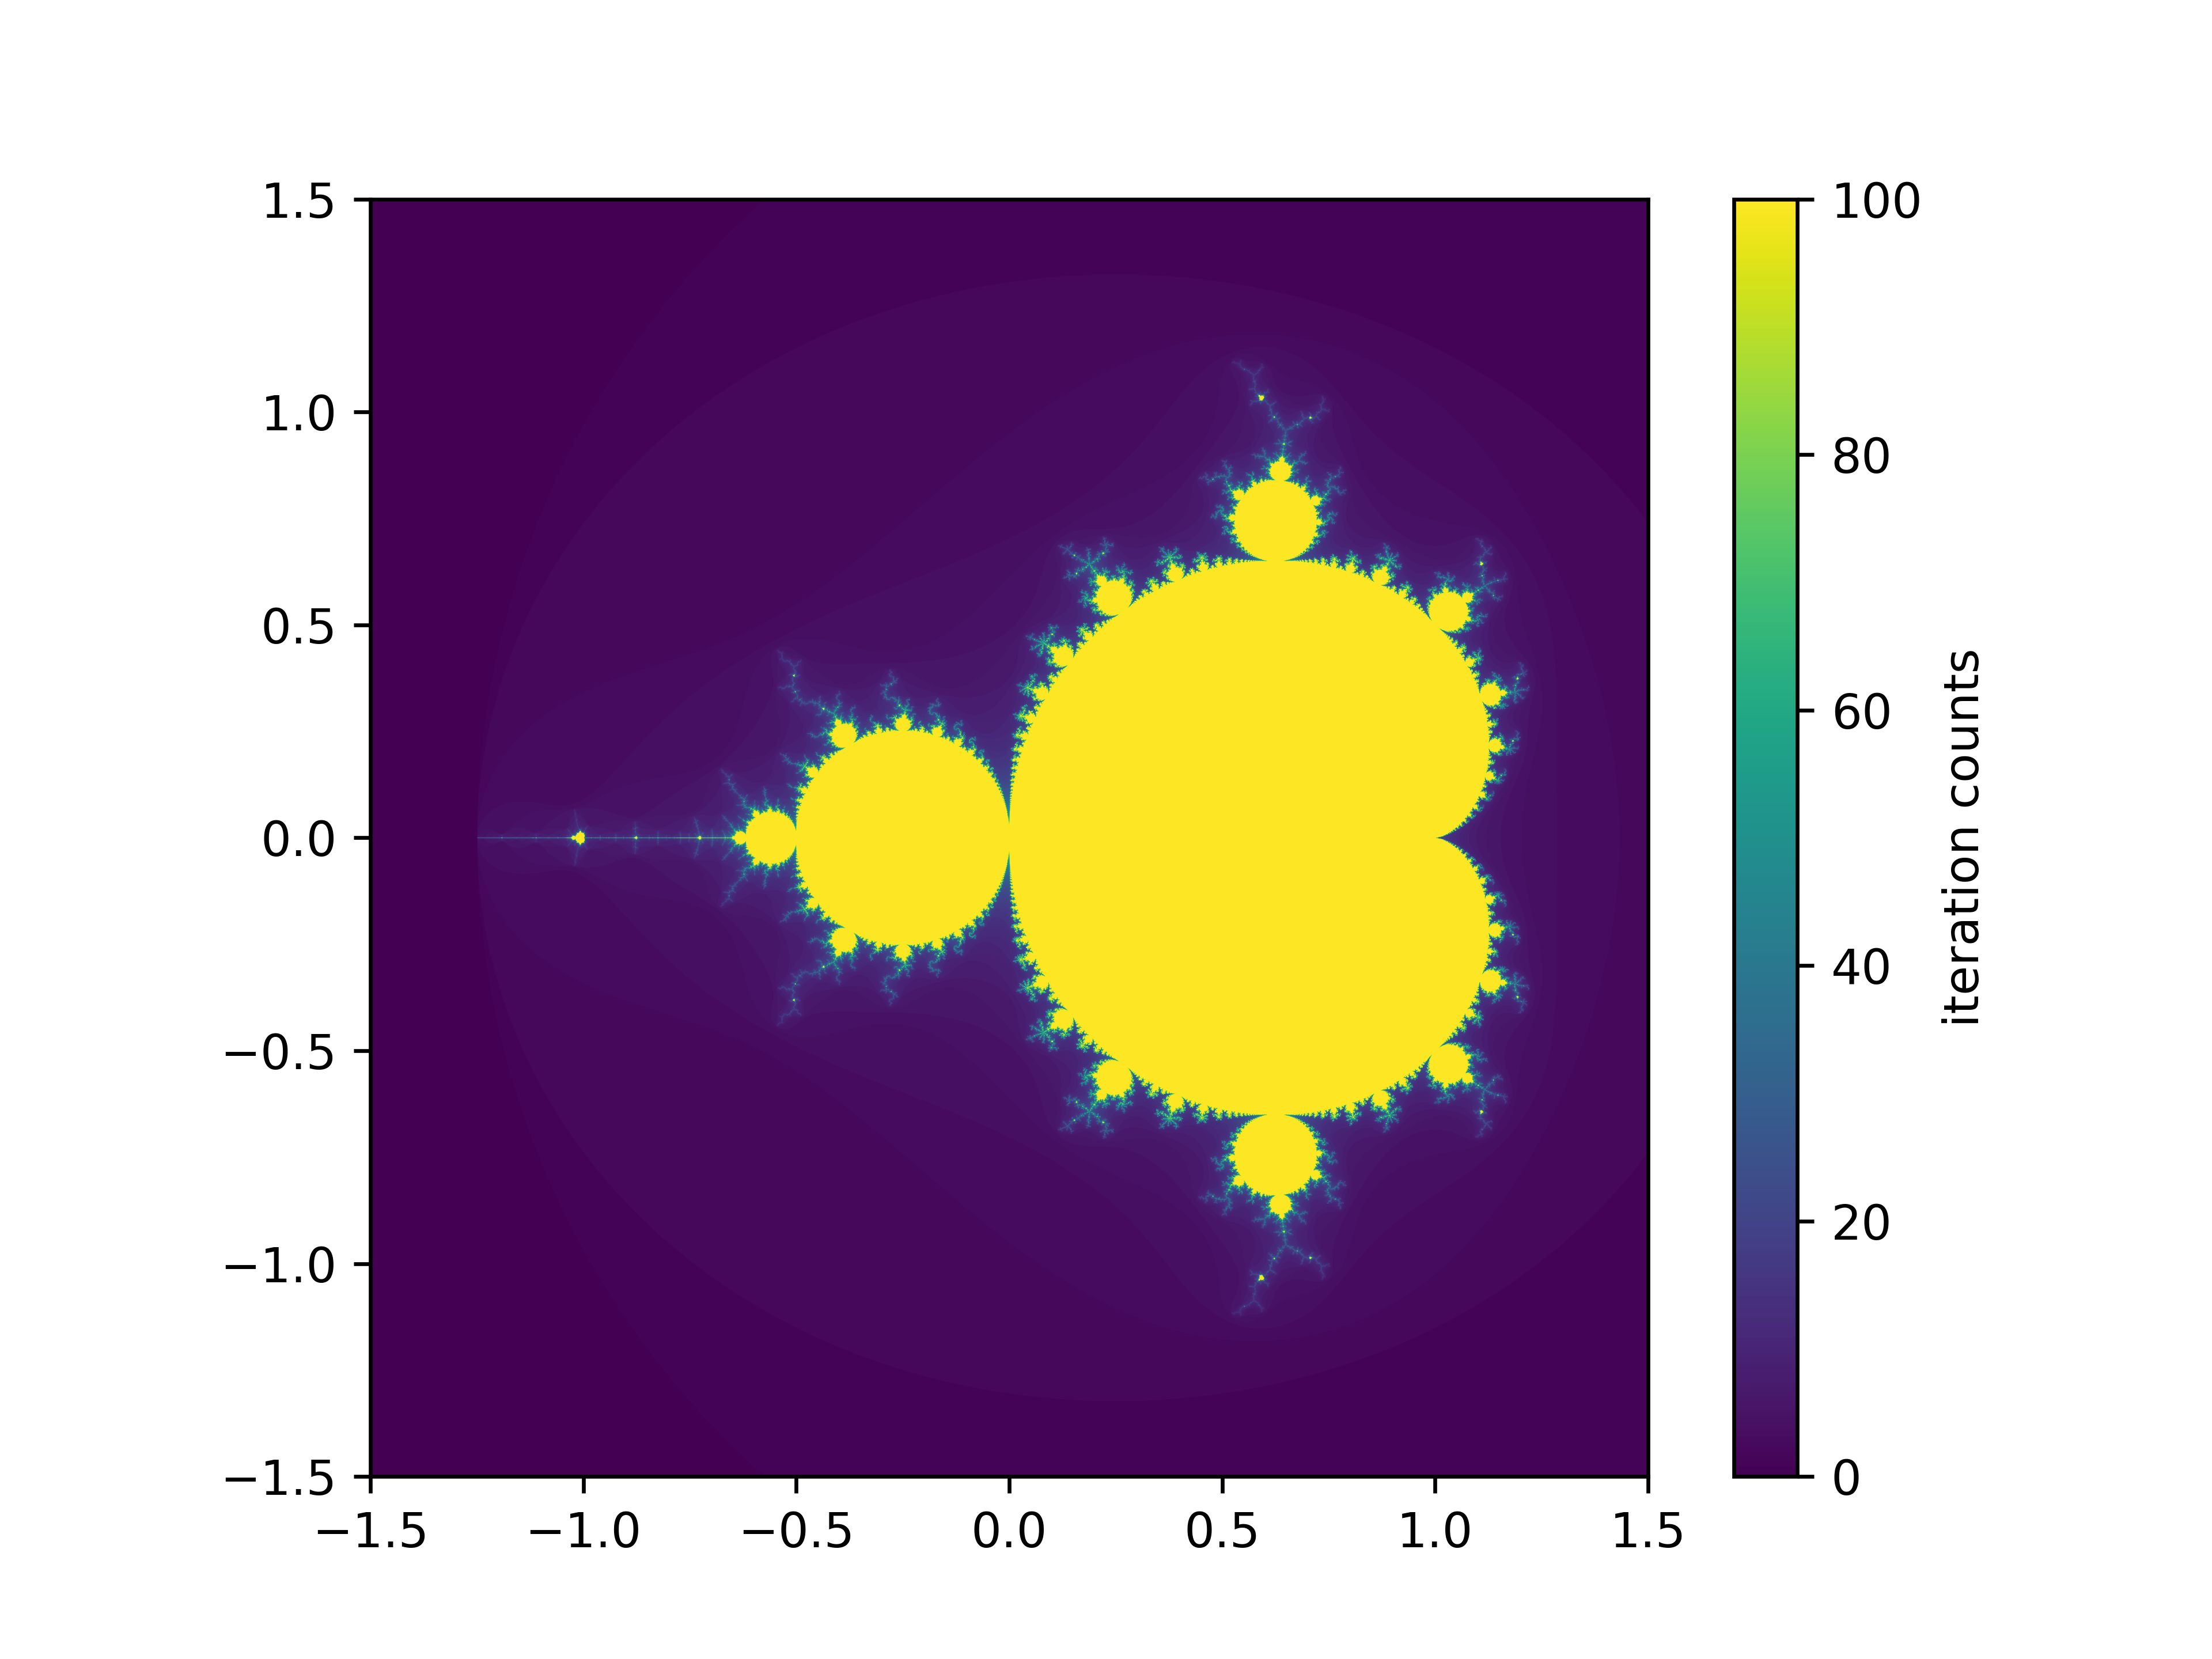
\includegraphics[width=.45\textwidth]{./png/man_color_n100.png}
	\caption{$N=100$,每迭代一次颜色反转或变化一点(线性)}
	\label{color}
\end{figure}

在以下的情形4,5中将会使$f$的值还与$z$产生关联,使得生成的图片具有更为特别的样式。
\item 令$f(n,z)=\ln(n+1)$与$\displaystyle f(n,z)=\frac{\ln(|z|^2)}{2^n}$:
\begin{figure}[H]
	\centering
	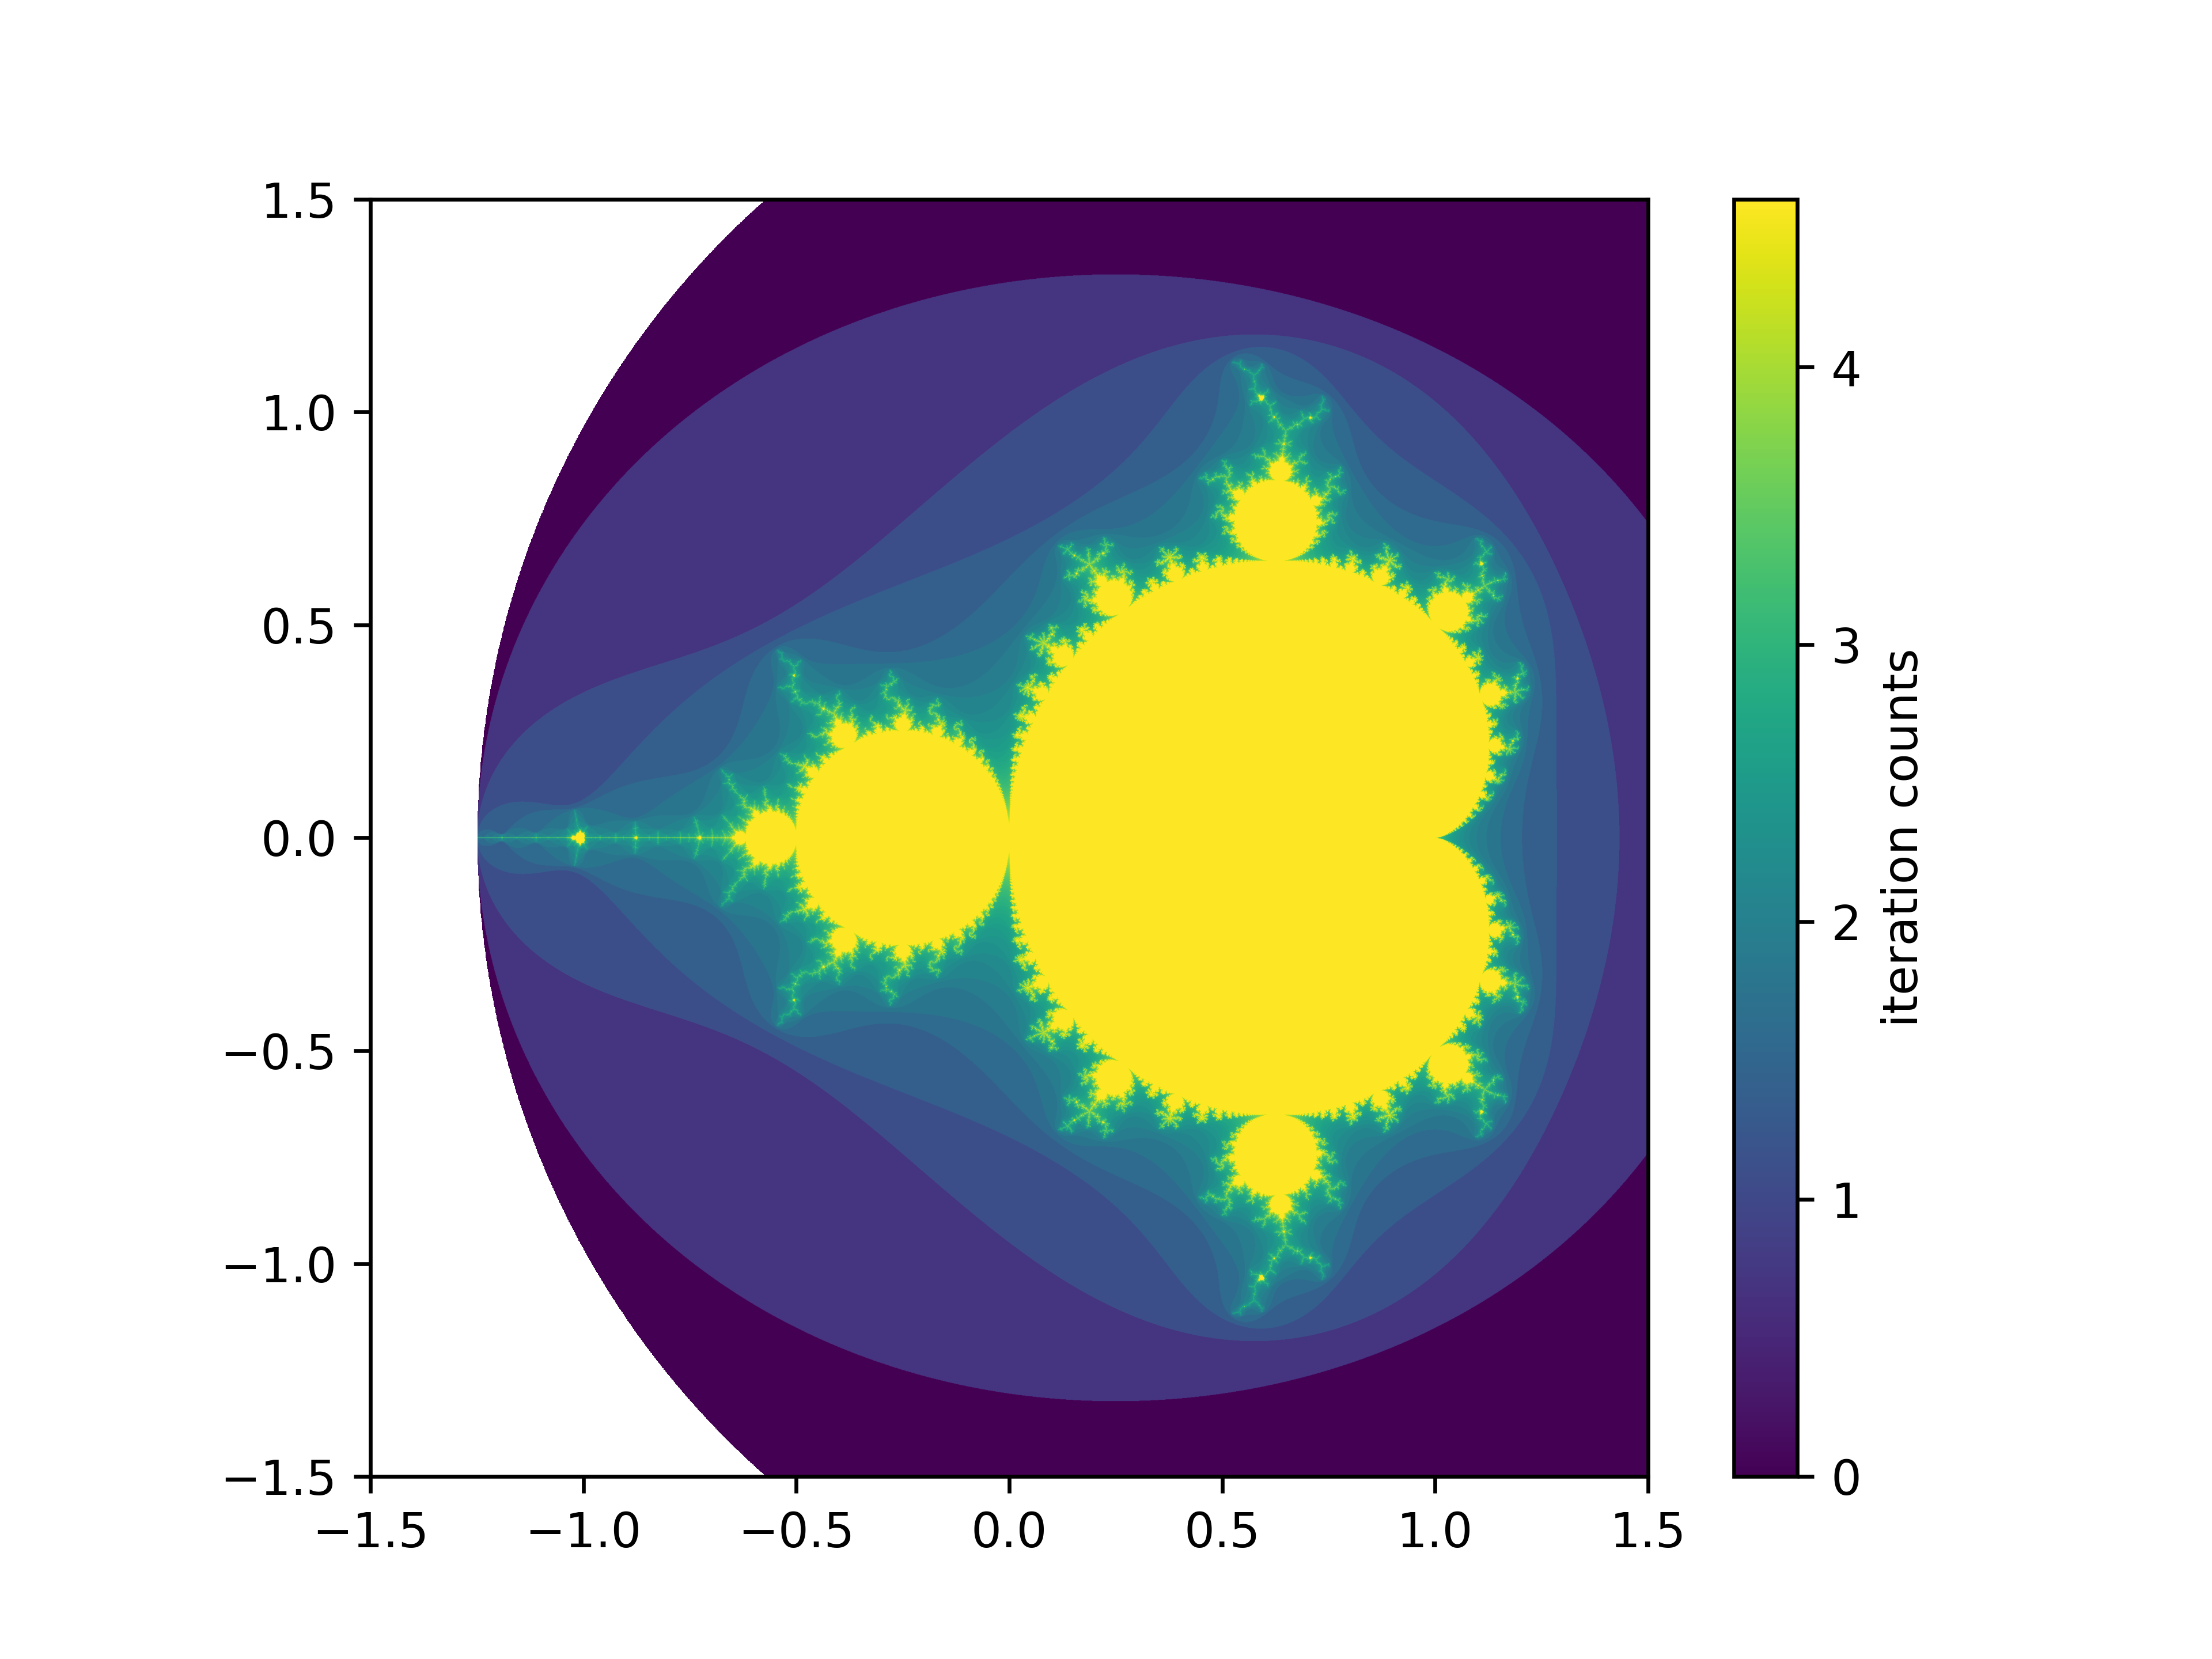
\includegraphics[width=.45\textwidth]{./png/man_colorln_n100.png}
	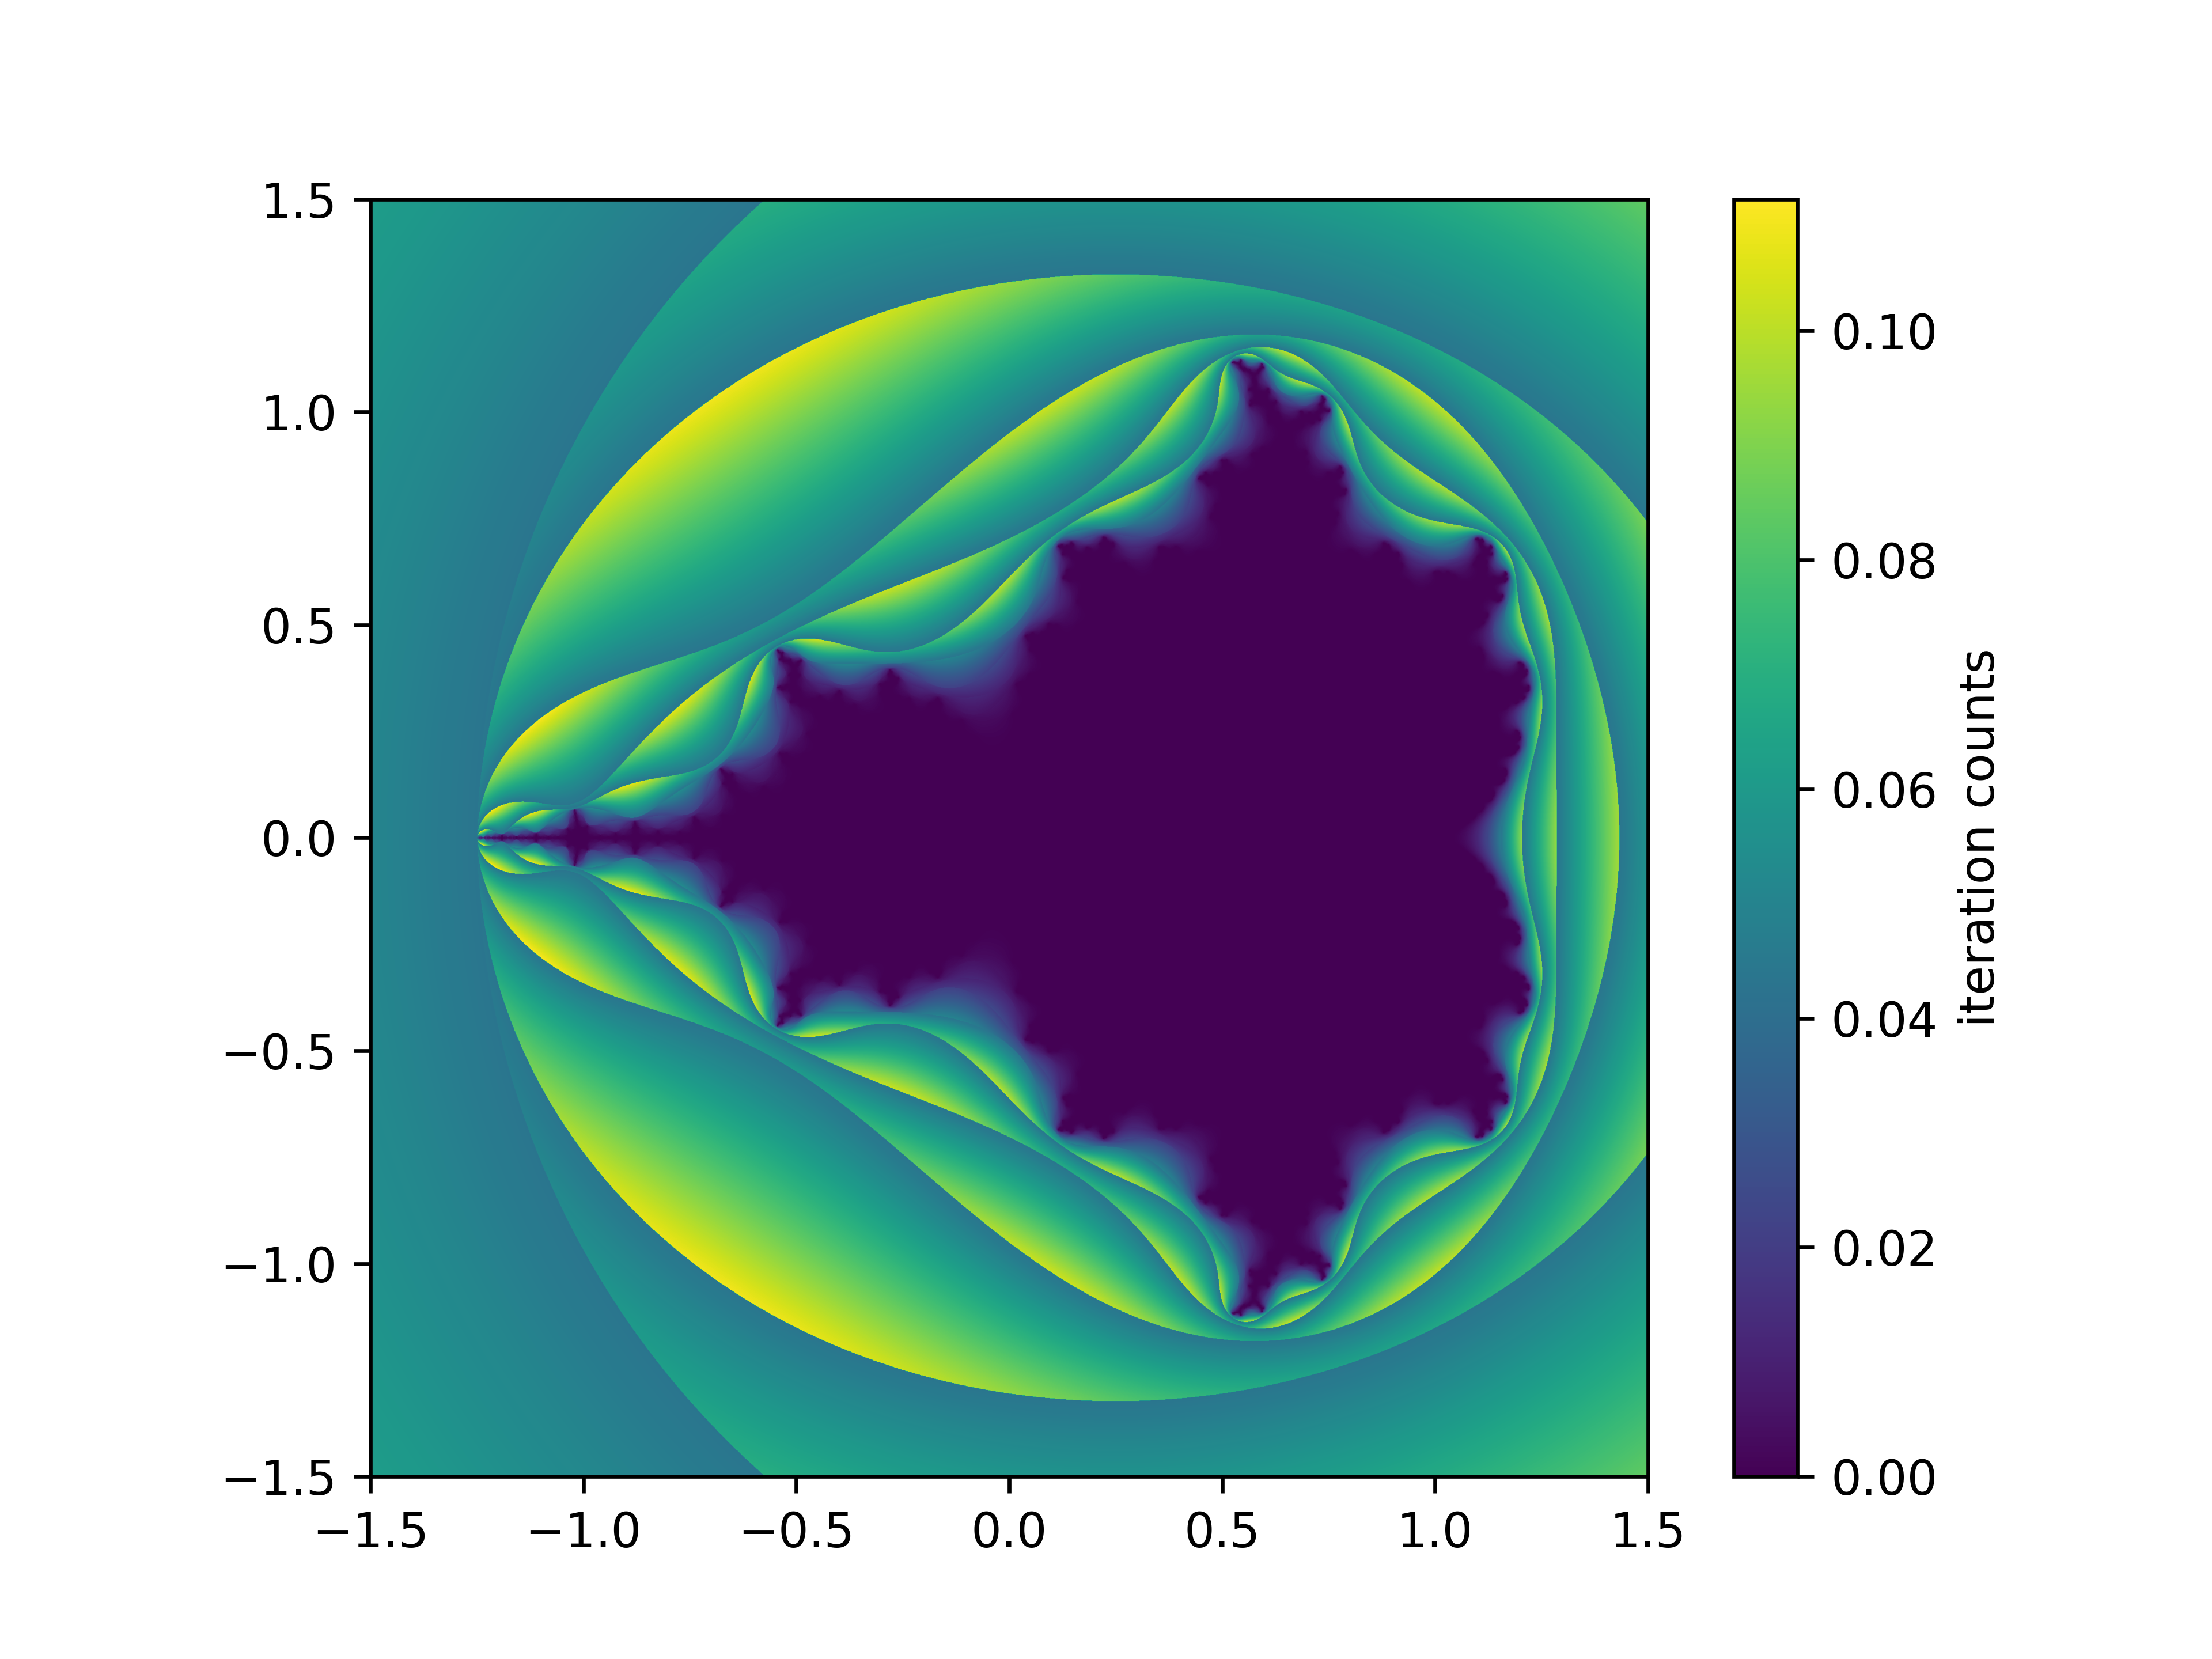
\includegraphics[width=.45\textwidth]{./png/man_colorlnx5-2_n100.png}
	\caption{$N=100$,每迭代一次颜色变化一点(对数)}
	\label{colorln}
\end{figure}
\item 令$f(n,z)=\sin(n)$与$\displaystyle f(n,z)=\sin(\ln(|z|^2))$:
\begin{figure}[H]
	\centering
	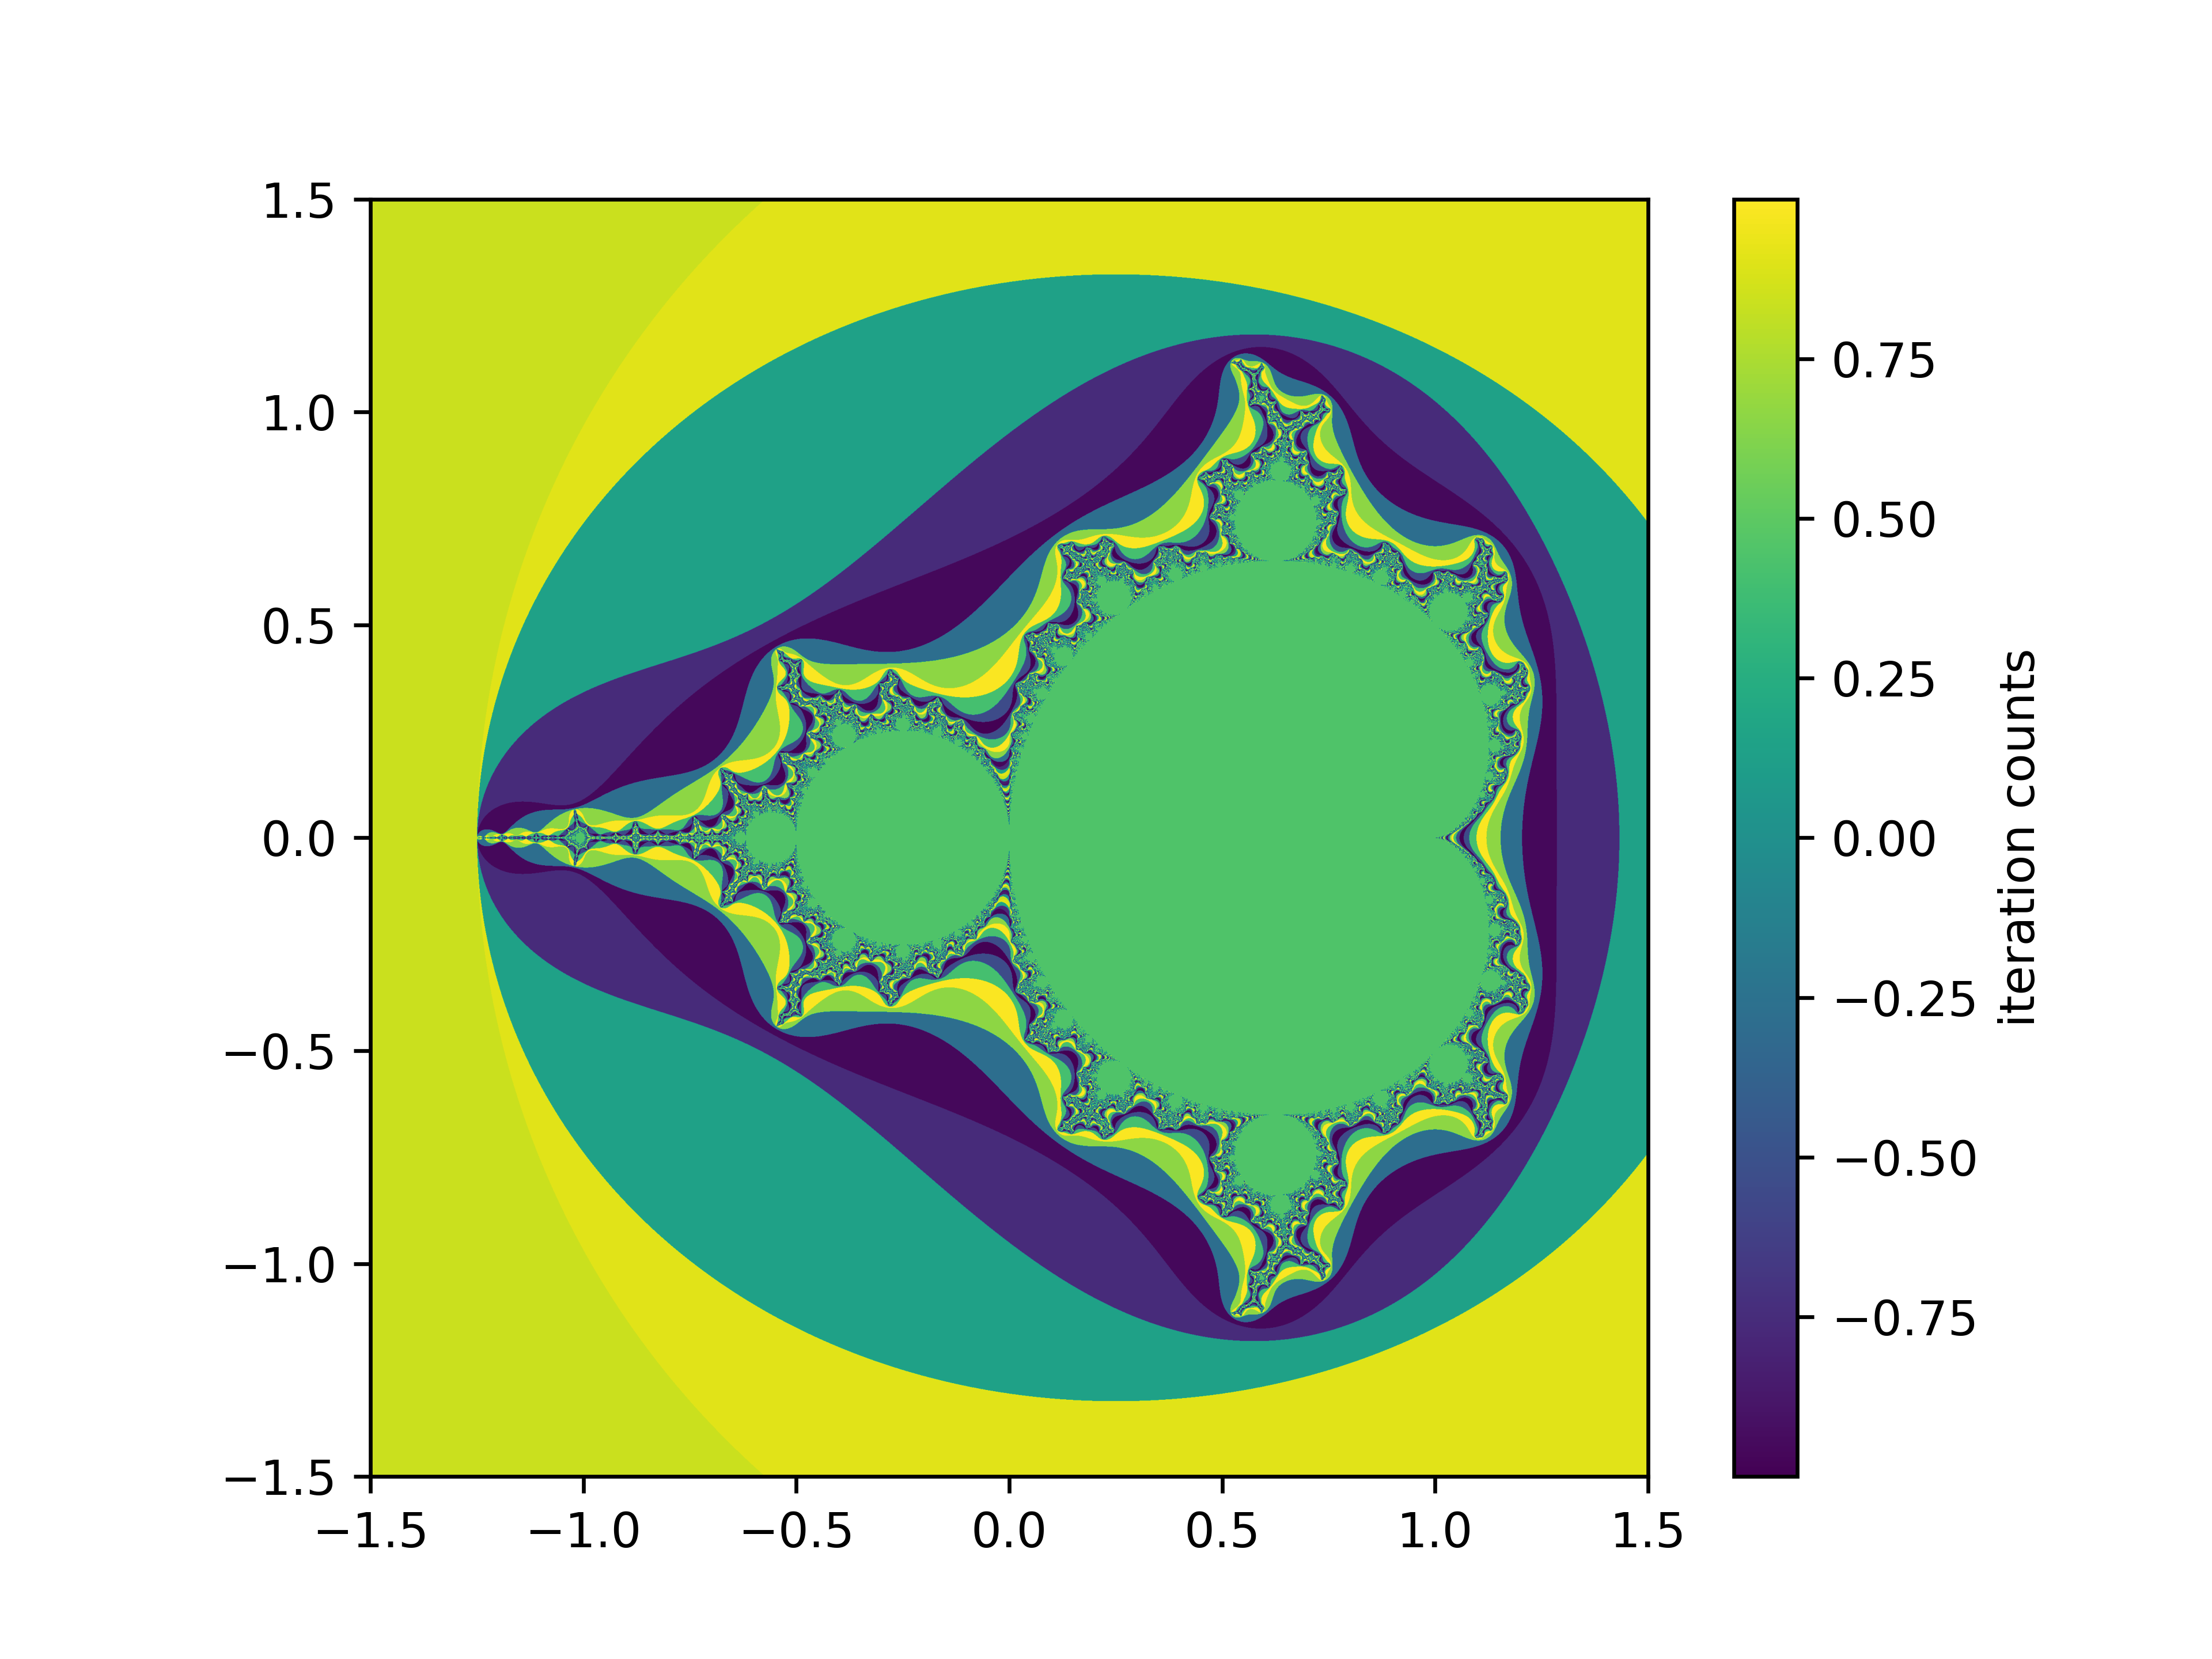
\includegraphics[width=.45\textwidth]{./png/man_colorsin_n100.png}
	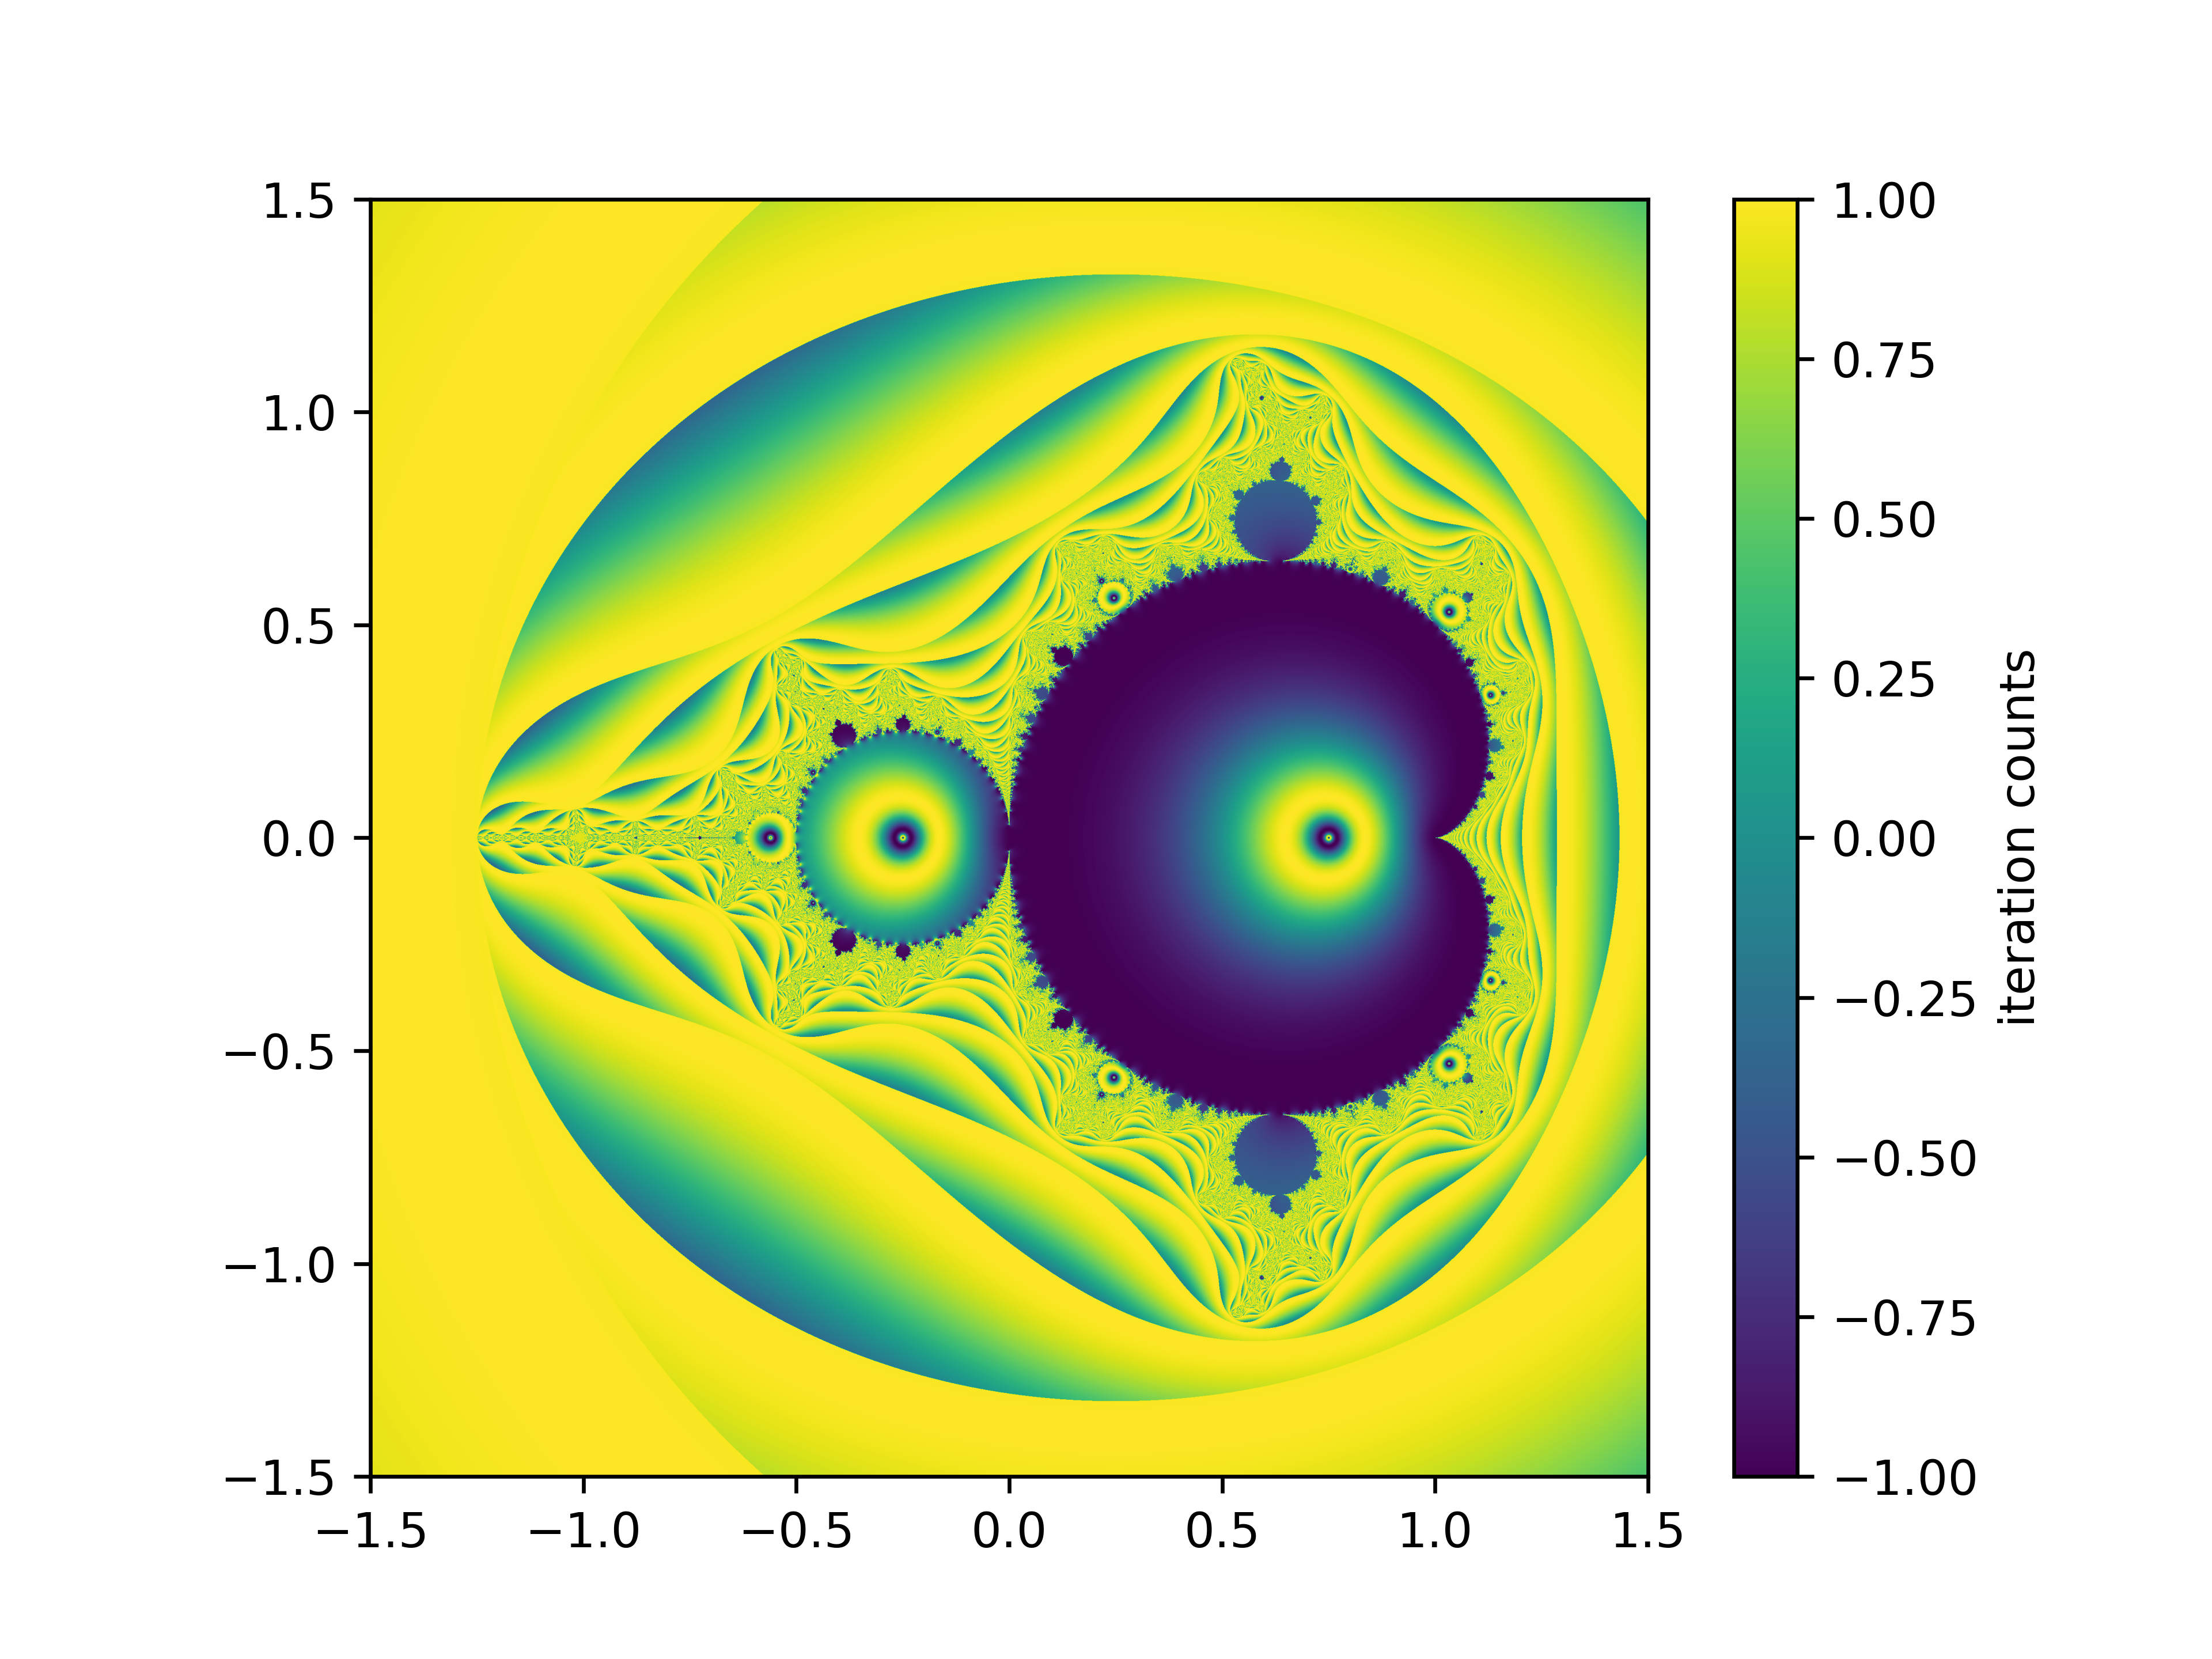
\includegraphics[width=.45\textwidth]{./png/man_colorsinlnx_n100.png}
	\caption{$N=100$,每迭代一次颜色变化一点(三角函数)}
	\label{colorsin}
\end{figure}
\end{enumerate}
\section{结论与思考}
通过以上的图像生成与探索的过程,我认识到了Mandelbrot Set的奇特与美妙之处。也使得我更为深入的思考,再继续改变函数$f(n,z)$,又会生成什么样的图形呢?我相信这件事值得我更进一步地查找资料与深入探索,并从中探索出更为美丽的数学世界。
\clearpage
	
\bibliographystyle{plain}
\bibliography{mandelbrot.bib}
	
\end{document}
%文档问题总结:
%1.图片的排版不够合理
%2.使用图片的大小较大使得文档整体体积较大
%3.对头文件的内容和使用还不够了解
%4.没有在一些重要部分将字体加粗
